\ProvidesFile{thesis.tex}[2021-02-05 PurdueThesis template file]

%
%  Process this using lualatex instead of pdflatex because of the
%  Feynman diagrams in the "Physics" appendix.
%
%  This is the root file for a simple example thesis.
%  This example can also be used to prepare a dissertation.
%
%  This thesis contains Feynman diagrams in the ap-physics.tex file.
%  For these to be processed correctly you must use the lualatex
%  program.  If your thesis doesn't have Feynman diagrams use pdflatex
%  instead of lualatex.
%  To make a final copy of your thesis put a '%'
%  in front of the \includeonly command and run:
%    lualatex thesis
%    lualatex thesis
%    lualatex thesis
%    biber thesis
%    makeindex thesis
%    lualatex thesis
%    lualatex thesis
%  Running Overleaf on your thesis file should do all of this
%  automatically.
%
%  References cited below:
%
%    TM2006 is short for Thesis Manual 2006.
%    ``A Manual for the Preparation of Graduate Theses'',
%    seventh revised edition, The Graduate School, Purdue University, 2006.
%    http://www.purdue.edu/GradSchool/documents/thesis/graduate-thesis-manual.pdf
%
%  Search for ``CHANGE'' below and change things as necessary.
%  I recommend putting ``%%'' before any existing lines that
%  need to be changed and adding your new line(s) immediately
%  below the existing lines.
%

% The kvoptions-patch package does not work in the 2020 version of
% LaTeX.  Do not try to use it.  Instead change any spaces ( ) in the
% \documentclass parameter values to at signs (@).
%
% (If/when the kvoptions-patch package is fixed, all at sign (@)
% characters can be changed back to space ( ) characters and the
%     \RequirePackage{kvoptions-patch}
% command uncommented.)
%
% See
%     Enter \documentclass parameters
% at
%     https://engineering.purdue.edu/~mark/PurdueThesis/#enter
% for instructions on how to fill in the \documentclass parameters.
% Remember to change all space ( ) characters in the values to
% at sign (@) characters.
\documentclass
[
  % Required parameters.
  institution = {Purdue@University},
  campus      = {West@Lafayette},
  program     = {Electrical@and@Computer@Engineering},
  degree      = {Doctor@of@Philosophy},
  author      = {Mark@Senn},
  document    = {A@Dissertation},
  graduation  = {May@2021},
  title       = {This@is@a@very@very@very@very@very@very@very@very@very@very@very@very@very@long@Title@of@the@Thesis},
  % Optional parameters.
  gridlines   = {true},
  marginlines = {false},
  timestamp   = {true},
]
{PurdueThesis}

% PurdueThesis.cls loads the rotating package which loads the graphicx
% package.  From
%     Packages in the `graphics' bundle
% at
%     http://ftp.math.purdue.edu/mirrors/ctan.org/macros/latex/required/graphics/grfguide.pdf
% on page 12
%     \graphicspath{<dir-list>}
%         This optional declaration may be used to specify a list of
%         directories in which tosearch for graphics files.  The
%         format is the same as for the LATEX 2e primitive\input@path.
%         A list of directories, each in a{}group (even if there is
%         only one in the list).  For
%         example:\graphicspath{{eps/}{tiff/}}would cause the system
%         to look in the subdirectories eps and tiff of the
%         currentdirectory.  (All modern TeX systems use / as the
%         directory separator, even on Windows.)   The default setting of
%         this path is \input@path that is: graphics files will be found
%         whereever TeX files are found.
%
% Look in the "graphics" subfolder for graphics files.
% This is done to reduce the number of files in the main thesis folder
% so the ones in there are easier to find.
\graphicspath{{graphics/}}

% Look in the "packages" subfolder for packages.
% This is done to reduce the number of files in the main thesis folder
% so the ones in there are easier to find.
\makeatletter
  \def\input@path{{packages/}}
\makeatother

%
% Configure bibliography.
%
% Automatically configure the bibliography.  Based on the
% institution, campus, and program listed in the \documentclass
% command \bibprocessor is set to "biblatex" or "bibtex".
% For biblatex, a
%    \usepackage[...]{biblatex}
% is done.  Put your bibliography entries in all-biblatex.bib.
% For bibtex, a
%     \bibliographystyle{...}
% command is done.  Put your bibliography entries in all-bibtex.bib.
%
% All combinations of institution, campus, and program use biblatex.
% Exceptions that use bibtex:
%     o  "Purdue University", "West Lafayette", "Earth, Atmospheric,
%        and Planetary Sciences" uses the ametsoc2014 bibliography style.
%     o  "Purdue University", "West Lafayette", "Veterinary Clinical
%        Sciences" uses the ama bibliography style.
%
% To override the default choices picked by \ConfigureBibliography, change,
% for example,
%     \ConfigureBibliography
% to
%     % \ConfigureBibliography
%     \newcommand{\bibprocessor}{biblatex}
%     \usepackage[backend=biber, citestyle=apa, dashed=false, sortcites=true, style=apa]{biblatex}
%     \addbibresource{all-biblatex.bib}
\ConfigureBibliography

%
% This is only relevant if you are using biblatex.
%
% This is an example of how to ignore urldate fields in your .bib file.
% See the first complete example on page 201 of
%     https://mirrors.rit.edu/CTAN/macros/latex/contrib/biblatex/doc/biblatex.pdf
%
% If you don't want to ignore urldate fields,
% comment out (put "%" before) the next ten lines.
%
\ifthen{\equal{biblatex}{\bibprocessor}}
{
  \DeclareSourcemap{
    \maps[datatype=bibtex]{
      \map{
        \step[fieldset=urldate, null]
      }
    }
  }
}

% For chemical figures, \chemfig.
\usepackage{chemfig}

% For \VerbatimInput.
\usepackage{fancyvrb}
  % https://andreas.scherbaum.la/blog/archives/670-Read-number-lines-in-a-file-in-LaTeX.html
  % Indent verbatim by 23.5pt so line numbers are within margin.
  \makeatletter
    \@totalleftmargin=23.5pt
  \makeatother
  
% For chemical equations.
% See
%     https://ctan.org/pkg/mhchem?lang=en
% From the "Package documentation" linked-to document
%     mhchem needs a couple of other packages.
%     For instance, expl3, amsmath and calc.
\usepackage[version=4]{mhchem}
  % If I'm loading the package to just define a few new commands I'll indent
  % two spaces right after loading the package and define the few new
  % commands here.  If I'm defining more than a few commands I usually do it
  % after loading all the packages.
  % Define "\nitrate" to be the chemical symbol for nitrate.
  \newcommand{\nitrate}{\ce{NO3{-}}}
  % Define "\pnitrate" (short for "parenthesized nitrate") to be the chemical
  % symbol for nitrate surrounded by parentheses.
  \newcommand{\pnitrate}{(\nitrate)}
  % "Define \vpnitrate" (short for "verbose parenthesized nitrate") to be
  % the word "nitrate" followed by a space followed by the chemical symbol
  % for nitrate with parentheses around it.
  \newcommand{\vpnitrate}{nitrate (\nitrate)}

% For
%     \cancel  
%     \highlight
% See
%     http://ftp.math.purdue.edu/mirrors/ctan.org/macros/latex/contrib/siunitx/siunitx.pdf
% pages 11--12.  
\usepackage{cancel}
  
% This gets rid of
%     [5] (./thesis.toc
%     ! Undefined control sequence.
%     \vbox_set:Nn ...box:D {\color_group_begin: #2\par 
%                                                       \color_group_end: }
%     l.32 ...}Basic Circuit Components}{31}{section.67}
%                                                       %
%     ? 
% and
%     [6]
%     ! Undefined control sequence.
%     \vbox_set:Nn ...box:D {\color_group_begin: #2\par 
%                                                       \color_group_end: }
%     l.61 ...rline {P.1}Frenchspacing}{67}{section.445}
%                                                       %
%     ?
% errors.
% See
%     https://github.com/latex3/latex2e/issues/73
\usepackage{etoc}

% For \setmaxprintline.
% \usepackage{hardwrap}

% For indexing.  Making an index is optional.
% Make these commands available:
%     COMMAND           DESCRIPTION
%     \index{string}    put "string" in index information
%     \makeindex        save information to make the index
%     \printindex       print the index
% See
%     https://ctan.org/pkg/makeidx?lang=en
% for more information.
\usepackage{makeidx}
  % By default \index ignores its argument.
  % This activates indexing.
  \makeindex
  % The "chapter name" for the index.
  \renewcommand{\indexname}{INDEX}

% For TeX, LaTeX, METAFONT, METAPOST, etc. related logos.
% This includes all the logos in the dtk-logos package, see
%     http://mirrors.ctan.org/macros/latex/contrib/hologo/hologo.pdf
% plus some extra definitions I made in pa-logos.sty.
\usepackage{pa-logos}

% For typographical conventions stuff including
%     \Emph{...}
%     \First{...}
%     \Keys{...}
%     \Literal{...}
%     \Menu{...}
%     \Place{...}
%     \Shell{...}
\usepackage{pa-typographic-conventions}

% For FloatBarrier.
% Put \FloatBarrier to process all unproccesed floats (tables and figures).
\usepackage{placeins}

% The mathtools package
% (see http://mirror.utexas.edu/ctan/macros/latex/required/amsmath/amsmath.pdf)
% loads the amsmath package which defines the
%     align
%     align*
%     alignat
%     alignat*
%     equation
%     equation*
%     flalign
%     flalign*
%     gather
%     gather*
%     multitaper
%     multitaper*
%     split
% environments and extends amsmath by defining many other commands.
% See
%     https://ctan.org/pkg/amsmath
% for information about amsmath and
%     http://ctan.math.washington.edu/tex-archive/macros/latex/contrib/mathtools/mathtools.pdf
% for information about mathtools.
\usepackage{mathtools}

% Follow ISO 80000-2:2019
%     o   put e, i, and pi in upright font automatically
%     o   use, for example, "\di x" to get "\,mathrm{d}\/x"
% This loads
%     o   amsmath.sty (which is already loaded above)
%     o   mathtools.sty
%     o   upgreek.sty
% Load the package.
\usepackage{pa-mismath}
  % Tell mismath that e, i, j, and pi in upright font automatically.
  \enumber
  \inumber
  \jnumber
  \pinumber
  % To typeset math italic e, i, j, and pi use
  %     \mathit e
  %     \mathit i
  %     \mathit j
  %     \itpi

% Define \includemedia.
\usepackage{media9}

% Define ``multicols'' environment environment used in demo-multicols.tex.
% CHANGE NEXT LINE?
\usepackage{multicol}

% For \ditto command.
\usepackage{pa-ditto}

% For \DigitDash---a dash the width of a digit in the current font.
\usepackage{pa-figure-dash}

% For \MyRepeat---????.
\usepackage{pa-repeat}






% For \textcent.
\usepackage{textcomp}
  
% !!! This doesn't work yet, figure it out later.
% For \textprimstress.
% \usepackage{tipa}

% Needed for chapter "Graphics", section "TikZ and PGF".
\usepackage{tikz}

% Needed for the Feynman diagram in ap-physics.tex.
% Tikz-feynman requires lualatex instead of pdflatex be run.
\usepackage[compat=1.1.0]{tikz-feynman}

% For \verbatiminput.
\usepackage{verbatim}

% The vertical space between a table heading and the table contents
% in a tabular environment.
\newcommand{\tabularspace}{\noalign{\vspace*{2pt}}}


% Define \I command so that \I1 does one \indent,
% \I2 does two \indents, etc.
\newcommand{\I}[1]{\MyRepeat{\indent}{#1}}

% My input without any output.
\newcommand{\MyI}{%
  \vbox{
    \fontsize{8}{10}\tt
    \VerbatimInput[
      firstnumber = 1,
      numbers     = left,
    ]{z.out}
  }
}  

% My input and output---not necessarily on the same page---but
% the input will all be on the same page.
\newcommand{\MyIO}{%
  \input{z.out}

  \vbox{
    \fontsize{8}{10}\tt
    \VerbatimInput[
      firstnumber = 1,
      numbers     = left,
    ]{z.out}
  }
}  

% My input and output---not necessarily on the same page---but
% the input will all be on the same page.
\newcommand{\MyIOS}{%
  \input{z.out}

  {%
    \fontsize{8}{10}\tt
    \VerbatimInput[
      firstnumber = 1,
      numbers     = left,
    ]{z.out}%
  }
}  

% My input and output together (on the same page).
\def\MyIOT{%
  \vbox{% no percent was here
    \input{z.out}% no percent was here
    % blark line was here
    \fontsize{8}{10}\tt
    \VerbatimInput[
      firstnumber = 1,
      numbers     = left,
    ]{z.out}% no percent was here
  }% no percent was here
}  

% Define \NL (newline) so LaTeX goes to the next output line.
% Just doing \\ complains
%     ! LaTeX Error: There's no line here to end.
% \mbox{} is an empty math box.
\newcommand{\NL}{\mbox{}\\}
% a walk around for the bug in lstlinebgrd
% https://tex.stackexchange.com/questions/451532/recent-issues-with-lstlinebgrd-package-with-listings-after-the-latters-updates
\makeatletter
\let\old@lstKV@SwitchCases\lstKV@SwitchCases
\def\lstKV@SwitchCases#1#2#3{}
\makeatother
\usepackage{lstlinebgrd}
\makeatletter
\let\lstKV@SwitchCases\old@lstKV@SwitchCases

\lst@Key{numbers}{none}{%
    \def\lst@PlaceNumber{\lst@linebgrd}%
    \lstKV@SwitchCases{#1}%
    {none:\\%
     left:\def\lst@PlaceNumber{\llap{\normalfont
                \lst@numberstyle{\thelstnumber}\kern\lst@numbersep}\lst@linebgrd}\\%
     right:\def\lst@PlaceNumber{\rlap{\normalfont
                \kern\linewidth \kern\lst@numbersep
                \lst@numberstyle{\thelstnumber}}\lst@linebgrd}%
    }{\PackageError{Listings}{Numbers #1 unknown}\@ehc}}
\makeatother

\definecolor{LightCyan}{rgb}{0.88,1,1}

\definecolor{codegreen}{rgb}{0,0.6,0}
\definecolor{codegray}{rgb}{0.5,0.5,0.5}
\definecolor{codepurple}{rgb}{0.58,0,0.82}
\definecolor{backcolour}{rgb}{1.0,1.0,1.0}

\lstdefinestyle{mystyle}{
    backgroundcolor=\color{backcolour},
    commentstyle=\color{codegreen},
    keywordstyle=\color{magenta},
    numberstyle=\tiny\color{codegray},
    stringstyle=\color{codepurple},
    basicstyle=\footnotesize\ttfamily,
    breakatwhitespace=false,
    frame=single,
    numbers=left,
    xleftmargin=0em,
    breaklines=true,
    captionpos=b,
    keepspaces=true,
    showspaces=false,
    showstringspaces=false,
    showtabs=false,
    tabsize=2,
    belowskip=1em,
}
\lstset{style=mystyle}


% Print a list of files used and their version numbers in the log file.
\listfiles


\begin{document}

\maketitle

% Front matter:
%     dedication
%     acknowledgments
%     preface
%     table of contents
%     list of tables
%     list of figures
%     list of symbols
%     abbreviations
%     nomenclature
%     glossary
%     abstract
\include{ch-front}

%
% Put chapter \include commands here.
%

% Introductions may precede the first chapters or major divisions of theses.
% Reference: TM2006, page 31.
% CHANGE NEXT LINE?
\ProvidesFile{ch-introduction.tex}[2021-01-04 introduction chapter]

\chapter{INTRODUCTION}

Draizelle Sexon \cite{sexon2012} recommends using these chapter names:\\
\I2 Problem and Its Background\\
\I2 Review of Related Literature and Studies\\
\I2 Methodology of the Study\\
\I2 Presentation, Analysis and Interpretation of Data\\
\I2 Summary, Conclusions, and Recommendations

Mantian Xue's \cite{xue2019} thesis contained these chapters:\\
\I2 Introduction\\
\I2 Device Technology\\
\I2 Graphene-based Biosensors\\
\I2 Graphene-based Ion Sensing\\
\I2 MoS${}_2$-based Sensors\\
\I2 Conclusion and Future Work

I suggest thinking carefully about the structure of your thesis
and using appropriate chapter names.


\section{English-related information}

\subsection{Typographic Conventions}

{
  \newlength{\Parindent}
  \setlength{\Parindent}{\parindent}
  \newcommand{\Indent}{\advance\leftskip by \Parindent}
  \parindent = 0pt

  \newcommand{\Describe}[2]{%
    {\Indent \Indent #1\endgraf}%
    {\Indent \Indent \Indent #2\endgraf}%
  }

  {\Indent The following typographic conventions are used in this document.
    These conventions were influenced by \cite{wireshark-users-guide,dijk2000,weh2016}.\endgraf}

  % Admonitions information is in \cite{wireshark-users-guide}.
  % Admonitions are not supported yet.

  % Dialog and window buttons information is in \cite{wireshark-users-guide}.
  % Dialog and window buttons are not supported yet.

  \Describe
  {\Emph{Emphasis}, \First{First Use}, and \Title{Title}}
  {%
    Emphasis: You \Emph{must} do this.\\
    First Use: The first use of an unusual term is \First{emphasized}.
    It is defined soon after it is emphasized.
    The sensor was installed in an \First{ekayak}.
    An ekayak is an electric kayak,
    we used a Duke Energy model
    % A digit dash is used to separate digits---it's the same width as a digit.
    % From http://everets.org/kevin/ten-codes.php retrieved on 2020-02-28:
    %     CODE  MEANS
    %     10-7  Out of service
    % So, the model number is a joke.
    10\FigureDash 7
    for this research.\\
    Title: He read \Title{The Grapes of Wrath}
    and watched \Title{Citizen Kane}.%
  }

  \Describe
  {\Keys{Keyboard} \Keys{Keys}}
  {%
    \Keys{Control + A} means press the Control key and A key at the same time.
    \Keys{A} \Keys{B} means press key A and then press key B.%
  }

  \Describe
  % Can't use \verb iside an arguement to \Describe.
  {{\tt Literal Elements}}
  {%
    Literal elements include checkboxes,
    code,
    environment variables,
    file names,
    function names,
    \LaTeX\ input,
    output,
    variable names,
    and verbatim input (except for commands typed on the command line).
  }

  \Describe
  {\Menu{Menu > Items}}
  {%
    To make sure smooth scrolling is on go to
    \Menu{Open menu > Preferences}
    and make sure the
    {\tt Use smooth scrolling}
    checkbox is checked.%
  }

  \Describe
  {\Place{Placeholders}}
  {Placeholders need to be replaced with real input.}
  
  \Describe
  {\Shell{\ttfamily\bfseries shell commands}}
  {Commands typed on the command line by the user.}
  
}


\subsection{Logical punctation}

I use logical punctuation \cite{yagoda2011}:\\
  \I2 The sign said ``Buses Only''.\\
instead of\\
  \I2 The sign said ``Buses Only.''\\
so quoted material,
and only quoted material,
is inside quotes.
This is new and not many people use it.
Your major professor may not like this style.
Check with them before you decide to use this.


\subsection{Serial comma}

I use the serial comma:\\
  \I2 apple, berry, and cherry\\
instead of\\
  \I2 apple, berry and cherry\\
because I find it easier
to see the list items
when they are separated by commas.





I like
to start all chapter names with \verb+ch-+.
Chapter names are everything
from the beginning of the thesis through the last chapter.
Chapters include all front matter
in addition to all chapters.

Appendices start with \verb+ap-+ and are everything after the last chapter
including any bibliography,
colophon,
indices,
and vita.

Graphics files start with \verb+gr-+.

\LaTeX\ package files start with \verb+pa-+.


\section{\LaTeX-related information}

\subsection{Input reading rules}

\LaTeX\ uses the following rules when reading input:
\begin{itemize}
  \item the end of a line is equivalent to a space
  \item spaces at the beginning of a line are ignored
\end{itemize}

The itemize environment takes lots of space---sometimes
I like to compress the layuot as shown below.

\subsection{Input preparation conventions}

I've used \LaTeX\ over~30 years
and use these personal conventions
to prepare input.
Using these conventions leads
to many short lines,
but I find those easier
to read and edit.
Do whatever works best for you.

\I2 start input lines with\\
  \I3 the first word of a sentence\\
  \I3 \verb+(+\\
  \I3 \verb+and+\\
  \I3 \verb+but+\\
  \I3 \verb+or+\\
  \I3 \verb+to+

\NL
\I2 end input lines with\\
  \I3 sentence-ending periods\\
  \I3 phrase-ending commas\\
  \I3 phrase-ending colons\\
  \I3 phrase-ending semicolons\\
  \I3 \verb+)+\\
  \I3 \verb+\\[+\textit{dimension}\verb+]+\\
  \I3 \verb+\\+

\NL
\I2 put these on a line of their own\\
  \I3 \verb+\begin{+\textit{environment name}\verb+}+\\
  \I3 \verb+\end{+\textit{environment name}\verb+}+\\
  \I3 short parenthetical remark




% Summary and/or conclusions are optional but often used.
% The summary and/or conclusions often are the last
% the last major division(s) of the text.
% Reference: TM2006 page 32.
% CHANGE NEXT LINE?
\include{ch-summary}

% Recommendations are optional.
% You may include recommendations as a major division if your
% subject matter and research dictate.
% Reference: TM2006 page 32.
% CHANGE NEXT LINE?
\ProvidesFile{ch-recommendations.tex}[2021-01-04 recommedations chapter]

\chapter{RECOMMENDATIONS}

Buy low.
Sell high.


% Testing.
% This chapter should not be included in a normal thesis.
% Its purpose is to test doing some unusual things.
\ProvidesFile{ch-testing.tex}[2021-01-11 testing chapter]

{
  \makeatletter
    \renewcommand\@makechapterhead[1]{{%
      \renewcommand{\baselinestretch}{1} \reset@font
      \large\bf\thechapter. #1\endgraf
    }}

    \chapter{TEST CHAPTER---THIS IS A VERY, VERY, VERY, VERY, VERY, VERY, VERY, VERY, VERY, VERY LONG CHAPTER NAME}
  \makeatother
}

This is a footnote\footnote{This is a footnote.}

Cite a reference with a very, very, very, \ldots long title
\cite{test-long-title}.



% Print the bibliography.
\PrintBibliography


% Appendices are optional.
% Appendices are not necessarily a part of every thesis.
% An appendix is used for supplementary illustrative material,
% original data, computer programs, and other material that
% is not necessarily appropriate for inclusion within the
% text of your thesis.
% Reference: TM2006 page 33.
% Use ``\appendix'' for one appendix or ``\appendices'' for more than one
% appendix.
% CHANGE NEXT LINES AND LINES FOLLOWING IT?
\appendices

% My filename conventions:
%     FILE THAT START WITH    ARE
%     ap-                     appendices
%     ch-                     chapters
%     pa-                     packages
%     z                       temporary files

% For "About Appendices" appendix.
\include{ap-about-appendices}

% Check margins.
\ProvidesFile{ap-check-margins.tex}[2021-01-04 check margins appendix]

\begin{VerbatimOut}{z.out}
\chapter{CHECK MARGINS}
\end{VerbatimOut}

\MyIO


\begin{VerbatimOut}{z.out}

\MyRepeat{This is a sentence. }{300}
\end{VerbatimOut}

\MyIO


\begin{VerbatimOut}{z.out}
{
  \tiny
  \MyRepeat{This is a sentence. }{600}
}
\end{VerbatimOut}


% Citations.
\ProvidesFile{ap-citations.tex}[2021-01-04 citations appendix]

\begin{VerbatimOut}{z.out}
\chapter{CITATIONS}
\end{VerbatimOut}

\MyIO


% For \LaTeX\ answers I refer to
% \citetitle{lamport1994}
% and then to
% \citetitle{goossens1994}
% or
% \citetitle{kopka1999}.
% \citetitle{kopka1999}
% is an update to \citetitle{kopka1995} (the 1995 edition).

\begin{VerbatimOut}{z.out}
For \LaTeX\ answers I refer to
\cite{lamport1994}
and then to
\cite{goossens1994}
or
\cite{kopka1999}.
\cite{kopka1999}
is an update to \cite{kopka1995} (the 1995 edition).
\end{VerbatimOut}

\MyIO


Here is an example .bib file entry:

\begin{VerbatimOut}{z.out}
@misc{example2020,
  address   = {Imaginaryville, Indiana},
  author    = {Andrew Anteater and Bertha Bear and Charles Cheetah and Davida Deer and Ethan Eagle},
  date      = {2020-10-27},
  doi       = {00.0000/000-0-000-00000-0},
  editor    = {Mark Senn},
  edition   = {2},
  isbn      = {{000\FigureDash 0\FigureDash 000\FigureDash 00000\FigureDash 0}},
  publisher = {Bogus International Publishing Company},
  title     = {An Imaginary Document Not About {Mark Senn} or {NASA}},
  url       = {https://bogus.com/bogus.html},
  urldate   = {2020-10-27},
  version   = {1.0},
}
\end{VerbatimOut}

\MyI


Here are some example BibLaTeX citations.
Depending on the style being used these will produce different results.

\mbox{}\\
\begin{tabular}{@{}ll@{}}
  \bf Input&                        \bf Output\\
  \verb+\cite{example2020}+&        \cite{example2020}\\
  \verb+\cite*{example2020}+&       \cite*{example2020}\\
  \verb+\citeauthor{example2020}+&  \citeauthor{example2020}\\
  \verb+\citeauthor*{example2020}+& \citeauthor*{example2020}\\
  \verb+\citedate{example2020}+&    \citedate{example2020}\\
  \verb+\citetitle{example2020}+&   \citetitle{example2020}\\
  \verb+\citetitle*{example2020}+&  \citetitle*{example2020}\\
  \verb+\citeurl{example2020}+&     \citeurl{example2020}\\
  \verb+\citeyear{example2020}+&    \citeyear{example2020}\\
  \verb+\parencite{example2020}+&   \parencite{example2020}\\
  \verb+\textcite{example2020}+&    \textcite{example2020}\\
\end{tabular}


% Common mistakes.
\ProvidesFile{ap-common-mistakes.tex}[2021-01-04 common mistakes appendix]

\begin{VerbatimOut}{z.out}
\chapter{COMMON MISTAKES}

The following Headings, Mathematics, and Text
sections describe some common mistakes.


\section{Headings}

\ifthen{\equal{\bibprocessor}{biblatex}}
{\textcite[page~289]{farkas2011} }
\ifthen{\equal{\bibprocessor}{bibtex}}
{\cite{farkas2011} }
wrote

\begin{quotation}
  The practice of stacking headings
  is routinely condemned by style manuals
  and other authorities.
  Here is a typical statement,
  taken from Houghton Mifflin's guidelines for authors.
  \begin{quotation}
    Avoid ``stacking'' heads,
    or placing two levels
    of headings together without intervening text.
    A heading cannot substitute
    for the transitional
    or introductory paragraphs
    that guide the reader through a chapter.
    Remember too that a chapter opening looks better in type
    when one
    or more paragraphs
    of text precede the first heading.
  \end{quotation}
\end{quotation}
\end{VerbatimOut}

\MyIOT

\begin{VerbatimOut}{z.out}


\section{Mathematics}

\subsection{Put a little extra horizontal space before dx.}
\end{VerbatimOut}
\MyIO


\begin{VerbatimOut}{z.out}


\section{Text}
\end{VerbatimOut}

\MyIO


\begin{VerbatimOut}{z.out}

\subsection{e.g.}
\index{.e.g.,}

``e.g.'' should always be followed by a comma.
\end{VerbatimOut}

\MyIOT


\begin{VerbatimOut}{z.out}

\subsection{``et al.'' is an abbreviation}
\index{et al.}

The phrase ``et al.''
is an abbreviation
and should always be followed by a period.
It should be in the normal font for your document---%
do not italicize or underline it.

Example:\\[6pt]
\indent\indent
\begin{tabular}{@{}ll@{}}
  input&   \verb+Thun et al.~used data from Santa Claus.+\\
  output&  Thun et al.~used data from Santa Claus.\\
  comment& my recommendation\\[6pt]
  input&   \verb+Thun et al. used data from Santa Claus.+\\
  output&  Thun et al. used data from Santa Claus.\\
  comment& too much space after period---\LaTeX\ thinks period is end of sentence\\[6pt]
  input&   \verb+Thun et al\@. used data from Santa Claus.+\\
  output&  Thun et al\@. used data from Santa Claus.\\
  comment& spacing is right but the ``et al.'' could occur at end of a line\\
\end{tabular}
\end{VerbatimOut}

\MyIOT


\begin{VerbatimOut}{z.out}

\subsection{i.e.}
\index{i.e.,}

``i.e.'' should always be followed by a comma.
\end{VerbatimOut}

\MyIO


% Defining commands.
\ProvidesFile{ap-defining-commands.tex}[2021-01-04 defining commands appendix]

\begin{VerbatimOut}{z.out}
\chapter{DEFINING COMMANDS}

The next paragraph demonstrates how to define and use a command.

\renewcommand{\t}[2]
{%
  Editors recommend that a #1 should never be
  followed by a #2 without some intervening text.
  I suggest writing for readers

}

\t{chapter title}{section heading}
\end{VerbatimOut}
\MyIO


% Demonstrate how to do separate appendices per chapter.
\include{ap-chapter-appendices}

% Demonstrate how to do separate references per chapter.
\include{ap-chapter-references}

% Figures.
\ProvidesFile{ap-figures.tex}[2021-02-04 figures appendix]

\begin{VerbatimOut}{z.out}
\chapter{FIGURES}

\end{VerbatimOut}

\MyIO


\begin{VerbatimOut}{z.out}

The
\verb+h+
specifier used in all the examples below
tells \LaTeX\ to put the figure
``here''
instead of trying
to find a good spot
at the top or bottom of a page.
Specifiers can be combined,
for example,
``\verb+\begin{figure}[htbp!]+''.
\end{VerbatimOut}

\MyIO


\begin{VerbatimOut}{z.out}

The complete list of specifiers:
\vspace*{6pt}
\begin{center}
  \begin{tabular}{@{}ll@{}}
    \toprule
    \bf Specifier& \bf Description\cr
    \midrule
    \noalign{\vspace*{2pt}}
    \tt b& bottom of page\cr
    \tt h& here on page\cr
    \tt p& on separate page of figures\cr
    \tt t& top of page\cr
    \tt !& try hard to put figure as early as possible\cr
    \bottomrule
  \end{tabular}
\end{center}
\end{VerbatimOut}

\MyIO


% !!!! Label ``fi:not-centered'' is ``\ref{fi:not-centered}''.
% !!!! Label ``sf:four-parts-c'' is ``\ref{sf:four-parts-c}''.

\begin{VerbatimOut}{z.out}

% MyRepeat is defined in MyRepeat.sty.
\MyRepeat{This is the first paragraph.  }{5}
\end{VerbatimOut}

\MyIO


\begin{VerbatimOut}{z.out}

\begin{figure}[ht]
  \includegraphics{gr-plot.pdf}
  \caption{%
    By default figures are not centered.
    This is a long caption to demonstrate that captions are single spaced.%
  }
  \label{fi:not-centered}
\end{figure}
\end{VerbatimOut}

\MyIO


\begin{VerbatimOut}{z.out}

\MyRepeat{This is the second paragraph.  }{10}
\end{VerbatimOut}

\MyIO


\begin{VerbatimOut}{z.out}

\begin{figure}[ht]
  \centering
  \includegraphics{gr-plot.pdf}
  \caption{Use {\tt \char'134centering\/} to center figures.}
  \label{fi:centered}
\end{figure}
\end{VerbatimOut}

\MyIO


\begin{VerbatimOut}{z.out}

\MyRepeat{This is the third paragraph.  }{15}
\end{VerbatimOut}

\MyIO


\begin{VerbatimOut}{z.out}

\begin{figure}[ht]
  \centering
  \includegraphics{gr-plot.pdf}
  \caption{This is another figuure.}
  \label{fi:another}
\end{figure}
\end{VerbatimOut}

\MyIO


\begin{VerbatimOut}{z.out}

\MyRepeat{This is the fourth paragraph.  }{10}
\end{VerbatimOut}

\MyIO


\begin{VerbatimOut}{z.out}
  
\begin{figure}[ht]
  \centering 
    \subcaptionbox
      {First subcaption.\label{sf:two-parts-a}}%
      [2in]%
      {\bfseries First subfigure.}%
    \hskip 0.5truein
    \subcaptionbox
      {Second subcaption.\label{sf:two-parts-b}}%
      [2in]%
      {\bfseries Second subfigure.}%
    \caption{This figure has two parts.}
    \label{fi:two-parts}
\end{figure}
\end{VerbatimOut}

\MyIO


\begin{VerbatimOut}{z.out}

\MyRepeat{This is the fifth paragraph.  }{10}
\end{VerbatimOut}

\MyIO


\begin{VerbatimOut}{z.out}
  
\newpage

\begin{figure}[ht]
  \centering
    \subcaptionbox
      {First subcaption.\label{sf:four-parts-a}}
      [2in]%
      {\bfseries First subfigure.}%
    \hskip 0.5truein
    \subcaptionbox
      {Second subcaption.\label{sf:four-parts-b}}
      [2in]%
      {\bfseries Second subfigure.}%
    \vspace*{\baselineskip}
    \subcaptionbox
      {Third subcaption.\label{sf:four-parts-c}}
      [2in]%
      {\bfseries Third subfigure.}%
    \hskip 0.5truein
    \subcaptionbox
      {Fourth subcaption.\label{sf:four-parts-d}}
      [2in]%
      {\bfseries Fourth subfigure.}%
  \caption{This figure has four parts.}
  \label{fi:four-parts}
\end{figure}
\end{VerbatimOut}

\MyIO


\begin{VerbatimOut}{z.out}

\MyRepeat{This is the sixth paragraph.  }{10}
\end{VerbatimOut}

\MyIO


\begin{VerbatimOut}{z.out}

\newpage

\begin{figure}[ht]
  \centering 
    % Use a 5" font.
    {\fontsize{5in}{5in}\selectfont\(\hspace*{-0.07em}\sqrt 2\)}
    \caption{%
      \LaTeX\ can make output big enough for T-shirts or posters.
      Square roots are printed with space before them,
      I put some negative horizontal space before this one to center it.%
    }
\end{figure}
\end{VerbatimOut}

\MyIO


\begin{VerbatimOut}{z.out}

\newpage

The remainder of this file tests having lots of figures.
There are 20 figures in this test.

\begin{figure}[ht]
  \centering
  \includegraphics[scale=0.1]{gr-plot.pdf}
  \caption{Use {\tt \char'134centering\/} to center figures.}
  \label{fi:centered}
\end{figure}

\begin{figure}[ht]
  \centering
  \includegraphics[scale=0.1]{gr-plot.pdf}
  \caption{Use {\tt \char'134centering\/} to center figures.}
  \label{fi:centered}
\end{figure}

\begin{figure}[ht]
  \centering
  \includegraphics[scale=0.1]{gr-plot.pdf}
  \caption{Use {\tt \char'134centering\/} to center figures.}
  \label{fi:centered}
\end{figure}

\begin{figure}[ht]
  \centering
  \includegraphics[scale=0.1]{gr-plot.pdf}
  \caption{Use {\tt \char'134centering\/} to center figures.}
  \label{fi:centered}
\end{figure}

\begin{figure}[ht]
  \centering
  \includegraphics[scale=0.1]{gr-plot.pdf}
  \caption{Use {\tt \char'134centering\/} to center figures.}
  \label{fi:centered}
\end{figure}

\begin{figure}[ht]
  \centering
  \includegraphics[scale=0.1]{gr-plot.pdf}
  \caption{Use {\tt \char'134centering\/} to center figures.}
  \label{fi:centered}
\end{figure}

\begin{figure}[ht]
  \centering
  \includegraphics[scale=0.1]{gr-plot.pdf}
  \caption{Use {\tt \char'134centering\/} to center figures.}
  \label{fi:centered}
\end{figure}

\begin{figure}[ht]
  \centering
  \includegraphics[scale=0.1]{gr-plot.pdf}
  \caption{Use {\tt \char'134centering\/} to center figures.}
  \label{fi:centered}
\end{figure}

\begin{figure}[ht]
  \centering
  \includegraphics[scale=0.1]{gr-plot.pdf}
  \caption{Use {\tt \char'134centering\/} to center figures.}
  \label{fi:centered}
\end{figure}

\begin{figure}[ht]
  \centering
  \includegraphics[scale=0.1]{gr-plot.pdf}
  \caption{Use {\tt \char'134centering\/} to center figures.}
  \label{fi:centered}
\end{figure}

\begin{figure}[ht]
  \centering
  \includegraphics[scale=0.1]{gr-plot.pdf}
  \caption{Use {\tt \char'134centering\/} to center figures.}
  \label{fi:centered}
\end{figure}

\begin{figure}[ht]
  \centering
  \includegraphics[scale=0.1]{gr-plot.pdf}
  \caption{Use {\tt \char'134centering\/} to center figures.}
  \label{fi:centered}
\end{figure}

\begin{figure}[ht]
  \centering
  \includegraphics[scale=0.1]{gr-plot.pdf}
  \caption{Use {\tt \char'134centering\/} to center figures.}
  \label{fi:centered}
\end{figure}

\begin{figure}[ht]
  \centering
  \includegraphics[scale=0.1]{gr-plot.pdf}
  \caption{Use {\tt \char'134centering\/} to center figures.}
  \label{fi:centered}
\end{figure}

\begin{figure}[ht]
  \centering
  \includegraphics[scale=0.1]{gr-plot.pdf}
  \caption{Use {\tt \char'134centering\/} to center figures.}
  \label{fi:centered}
\end{figure}

\begin{figure}[ht]
  \centering
  \includegraphics[scale=0.1]{gr-plot.pdf}
  \caption{Use {\tt \char'134centering\/} to center figures.}
  \label{fi:centered}
\end{figure}

\begin{figure}[ht]
  \centering
  \includegraphics[scale=0.1]{gr-plot.pdf}
  \caption{Use {\tt \char'134centering\/} to center figures.}
  \label{fi:centered}
\end{figure}

\begin{figure}[ht]
  \centering
  \includegraphics[scale=0.1]{gr-plot.pdf}
  \caption{Use {\tt \char'134centering\/} to center figures.}
  \label{fi:centered}
\end{figure}

\begin{figure}[ht]
  \centering
  \includegraphics[scale=0.1]{gr-plot.pdf}
  \caption{Use {\tt \char'134centering\/} to center figures.}
  \label{fi:centered}
\end{figure}

\begin{figure}[ht]
  \centering
  \includegraphics[scale=0.1]{gr-plot.pdf}
  \caption{Use {\tt \char'134centering\/} to center figures.}
  \label{fi:centered}
\end{figure}
\end{VerbatimOut}

\MyIO



% Graphics.
\ProvidesFile{ap-graphics.tex}[2021-01-04 graphics appendix]

\begin{VerbatimOut}{z.out}
\chapter{GRAPHICS}

There are many ways to make graphics for \LaTeX.
I like to use a system that uses \LaTeX\ fonts
so the appearance of the output is more professional.
\end{VerbatimOut}

\MyIOT


\begin{VerbatimOut}{z.out}

\section{Mathematica (Wolfram)}
\end{VerbatimOut}

\MyIOT


\begin{VerbatimOut}{z.out}

\section{MATLAB}
\end{VerbatimOut}

\MyIOT


\begin{VerbatimOut}{z.out}

\section{\METAPOST\ (uses \LaTeX\ fonts)}

I did this \METAPOST\ \cite{metapost} example
for Yanghyun Kim \cite{kim2009}.
\end{VerbatimOut}

\MyIOT


\begin{VerbatimOut}{z.out}

\newpage

\begin{figure}[ht]
  \centering 
    \subcaptionbox
      {\bfseries gr-kim1.pdf}%
      {\includegraphics{gr-kim1.pdf}}%
    \vskip 0.1truein
    \subcaptionbox
      {\bfseries gr-kim2.pdf}%
      {\includegraphics{gr-kim2.pdf}}%
    \caption{Graphics answers for Yanghyun Kim.}
\end{figure}
\end{VerbatimOut}

\MyIO


\begin{VerbatimOut}{z.out}

\section{R}
\end{VerbatimOut}

\MyIOT


\begin{VerbatimOut}{z.out}

\section{\TikZ\ and PGF (uses \LaTeX\ fonts)}
\end{VerbatimOut}

\MyIOT


\begin{VerbatimOut}{z.out}

\subsection{Clock}
\end{VerbatimOut}

\MyIOT


\begin{VerbatimOut}{z.out}

\begin{figure}[ht]
  \hbox to\textwidth{%
    \hfil
    \begin{tikzpicture}
      \def\CenterRadius{0.04cm}
      \def\InnerTickRadius{3.6cm}
      \def\OuterTickRadius{3.8cm}
      % Make \LR be an abbreviation for \LabelRadius so the
      % lines below will fit within the width of the page.
      \def\LabelRadius{4.5cm}      \let\LR=\LabelRadius
      \def\HourHandRadius{2.5cm}   \def\HourHandBase{0.3cm}
      \def\MinuteHandRadius{3cm}   \def\MinuteHandBase{0.4cm}
      \def\SecondHandRadius{3.5cm} \def\SecondHandBase{0.5cm}
      \def\DS{\displaystyle}
      \fill (0,0) circle (\CenterRadius);
      \foreach \i in {0,30,...,330}
      \draw (\i:\InnerTickRadius)--(\i:\OuterTickRadius);
      \node at (  0:\LR) {$\DS \qquad \sqrt9 + 9 - 9$};        %  3
      \node at ( 30:\LR) {$\DS \frac{9+9}9$};                  %  2
      \node at ( 60:\LR) {$\DS \frac{\sqrt9\sqrt9}9$};         %  1
      \node at ( 90:\LR) {$\DS 9 + \frac9{\sqrt9}$};           % 12
      \node at (120:\LR) {$\DS \frac{99}9$};                   % 11
      \node at (150:\LR) {$\DS 9 + \frac99$};                  % 10
      \node at (180:\LR) {$\DS \sqrt[\scriptstyle 9]{9^9}$};   %  9
      \node at (210:\LR) {$\DS 9 - \frac99$};                  %  8
      \node at (240:\LR) {$\DS 9 - \sqrt9 + \lceil.9\rceil$};  %  7
      \node at (270:\LR) {$\DS 9 - \frac9{\sqrt9}$};           %  6
      \node at (300:\LR) {$\DS \sqrt9\,! - \frac99$};          %  5
      \node at (330:\LR) {$\DS \sqrt9 + \frac99$};             %  4
      % In the following
      %   ABBREVIATION    DESCRIPTION
      %   deg             degrees
      %   min             minutes
      %   sec             seconds
      % for second hand:
      %   (9 sec/60 sec) * 360 deg = 54 deg;
      %   90 deg - 54 deg = 36 deg
      \draw[rotate around={36:(0,0)}]
        (-\SecondHandBase,\SecondHandBase) -- (\SecondHandRadius,0)
          -- (-\SecondHandBase,-\SecondHandBase) -- cycle;
      % for minute hand:
      %   (9 min/60 min) * 360 deg = 54 deg;
      %   90 deg - 54 deg = 36 deg
     \draw[rotate around={36:(0,0)}]
       (-\MinuteHandBase,\MinuteHandBase) -- (\MinuteHandRadius,0)
         -- (-\MinuteHandBase,-\MinuteHandBase) -- cycle;
      % for hour hand:
      %   (9 min * (60 sec/1 min)) + 9 sec) / 3600 sec
      %     = 549 sec / 3600 sec = 0.1525
      %   The hour hand is 0.1525 of the way from 9:00 to 10:00.
      %   Each hour is 30 degrees on the clock, so the hour hand
      %   position is
      %     30 deg * 0.1525 = 4.575 deg past 9:00
      %   180 deg - 4.575 deg = 175.425 deg
     \draw[rotate around={175.425:(0,0)}]
       (-\HourHandBase,\HourHandBase) -- (\HourHandRadius,0)
         -- (-\HourHandBase,-\HourHandBase) -- cycle;
    \end{tikzpicture}
    %    To make a one page clock document delete everything
    % below and add
    %     \end{document}
    \hfil
  }
  \caption{%
    The idea for this clock was originally from a
    Google+ posting by Afamefuna ``Ferdy'' Ibeabuchia.%
  }  
\end{figure}
\end{VerbatimOut}

\MyIOS


\begin{VerbatimOut}{z.out}

\subsection{Glider}
\end{VerbatimOut}

\MyIOT


\begin{VerbatimOut}{z.out}
  
\begin{figure}[ht]
  \hbox to\textwidth{%
    \hfil
    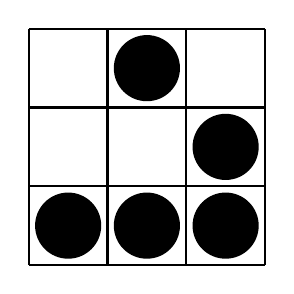
\begin{tikzpicture}[thick]
      \draw (0,0) grid (3,3);
      \foreach \c in {(0,0), (1,0), (2,0), (2,1), (1,2)}
        \fill \c + (0.5,0.5) circle (0.42);
    \end{tikzpicture}
    \hfil
  }
  \caption
  [%
    The glider
    is a pattern from the Game of Life,
    and it's used as an emblem representing the hacker community.%
  ]
  {%
    The glider \cite{hirzel2012}
    is a pattern from the Game of Life,
    and it's used as an emblem representing the hacker community.%
  }
\end{figure}
\end{VerbatimOut}

\MyIO


% Numbers and Units.
\include{ap-numbers-and-units}

% Resources.
\ProvidesFile{ap-resources.tex}[2021-01-04 resources appendix]

\begin{VerbatimOut}{z.out}
\chapter{RESOURCES}

From the
\href
  {https://journals.ieeeauthorcenter.ieee.org/your-role-in-article-production/ieee-editorial-style-manual/}%
  {IEEE Editorial Style Manuual}
  \cite{ieee-editorial-style-manual}:
\begin{itemize}
  \item
    The
    \href
      {http://journals.ieeeauthorcenter.ieee.org/wp-content/uploads/sites/7/IEEE-Editorial-Style-Manual_081920.pdf}%
      {IEEE Editorial Style Manual for Authors}
      \cite{ieee-editorial-style-manual-for-authors}
    contains a formal set of editorial guidelines.
  \item
    \href
    {http://journals.ieeeauthorcenter.ieee.org/wp-content/uploads/sites/7/Editing-Mathematics.pdf}%
    {Editing Mathematics}
    \cite{editing-mathematics}
    illustrates how to do mathematics.
  \item
    The
    \href
      {http://journals.ieeeauthorcenter.ieee.org/wp-content/uploads/sites/7/IEEE-Reference-Guide_081920.pdf}
      {IEEE Reference Guide}
    \cite{ieee-reference-guide}
    outlines how to cite references.
\end{itemize}

\end{VerbatimOut}

\MyIOS


% Tables.
\ProvidesFile{ap-tables.tex}[2021-01-04 tables appendix]

\begin{VerbatimOut}{z.out}
\chapter{TABLES}

\end{VerbatimOut}

\MyIOS


% \newlength{\ta}
% \newlength{\tb}
% \newlength{\tc}
% 
% \settowidth{\ta}{\vbox{\hbox{Money}\hbox{Market}}}
% \settowidth{\tb}{\vbox{\hbox{Stocks}\hbox{and}\hbox{Bonds}}}
% \settowidth{\tc}{\vbox{\hbox{Money}\hbox{Market}\hbox{and}\hbox{Stocks}}}
% 
% {
%     \renewcommand{\baselinestretch}{1}
%     \begin{table}
%       \caption{%
%         \hfil Allocation of the IRA and Keogh Wealth\hfil\break
%         \mbox{}\hfil for Investors With or Without Brokerage Accounts\hfil
%       }
%       \label{tab:ira}
%       \begin{center}
%         \begin{tabular}%
%           {%
%             |%
%             c%
%             |%
%             >{\centering\hspace{0pt}}m{\the\ta}%  Money Market
%             |%
%             c%                                    Stocks 
%             |%
%             c%                                    Bonds
%             |%
%             c%                                    Diversified
%             |%
%             >{\centering\hspace{0pt}}m{\the\tb}%  Stocks and Bonds
%             |%
%             >{\centering\hspace{0pt}}m{\the\tc}%  Money Market and Stocks
%             |%
%             c%                                    Others
%             |%
%           }
%           \hline
%           IMP&
%             Money Market&
%             Stocks&
%             Bonds&
%             Diversified&
%             Stocks and Bonds&
%             Money Market and Stocks&
%             Others\tabularnewline
%           \hline
%           1& 14.19\%& 57.71\%& 12.21\%& 4.50\%& 7.36\%& 3.04\%& 0.99\%\tabularnewline \hline
%           2& 14.08\%& 58.18\%& 12.32\%& 4.44\%& 7.30\%& 2.80\%& 0.88\%\tabularnewline \hline
%           3 &14.26\%& 58.09\%& 12.27\%& 4.50\%& 7.19\%& 2.75\%& 0.94\%\tabularnewline \hline
%           4 &13.94\%& 58.11\%& 12.14\%& 4.78\%& 7.35\%& 2.68\%& 0.99\%\tabularnewline \hline
%           5 &13.92\%& 58.13\%& 11.93\%& 4.56\%& 7.60\%& 2.98\%& 0.88\%\tabularnewline \hline
%         \end{tabular}
%       \end{center}
%       This table presents the allocations of the wealth in the IRA
%       and Keogh accounts in various asset classes.
%       Results from each set of imputed data are presented here.
%       The first column lists the number of the imputations,
%       and rest of the columns lists various allocations.
%       Entrees under each asset class show the percentage of investors
%       who have most of their IRA
%       and Keogh wealth invested in that particular asset class.
%       The asset class Diversified
%       includes stocks,
%       bonds,
%       and money market investments.
%       The asset class Others
%       include investments in various life insurance products,
%       annuities,
%       real estate, etc.
%       \medskip
%     \footnotesize SOURCE: Survey of Consumer Finances,
%     2001,
%     Federal Reserve Board,
%     USA.\par
%   \end{table}
% }


\begin{VerbatimOut}{z.out}

Here is a really simple table.

% "h" means put table "here"---don't let it float to top or bottom of page
\begin{table}[ht]
  \caption{The first three American Presidents.}
  \vspace*{6pt}
  \centering
    % Table format:
    %     WHAT    DESCRIPTION
    %     @{}     don't put extra space before first column
    %     r       right justify first column
    %     l       left justify second column
    %     @{}     don't put extra space after second column
    \begin{tabular}{@{}rl@{}}
      \toprule
      \bf Number& \bf Name\\
      \midrule
      1& George Washington\\
      2& John Adams\\
      3& Thomas Jefferson\\
      \bottomrule
    \end{tabular}
  \label{ta:first-three-american-presidents}
\end{table}
\end{VerbatimOut}

\MyIOS


\begin{VerbatimOut}{z.out}

\newpage

Here is the same table with a longer caption.

% "h" means put table "here"---don't let it float to top or bottom of page
\begin{table}[ht]
  \caption{%
    The first three American Presidents.
    This caption is
    much, much, much, much, much, much,
    much, much, much, much, much, much
    longer.%
  }
  \vspace*{6pt}
  \centering
    % Table format:
    %     WHAT    DESCRIPTION
    %     @{}     don't put extra space before first column
    %     r       right justify first column
    %     l       left justify second column
    %     @{}     don't put extra space after second column
    \begin{tabular}{@{}rl@{}}
      \toprule
      \bf Number& \bf Name\\
      \midrule
      1& George Washington\\
      2& John Adams\\
      3& Thomas Jefferson\\
      \bottomrule
    \end{tabular}
  \label{ta:first-three-american-presidents-longer-caption}
\end{table}
\end{VerbatimOut}

\MyIOS


\begin{VerbatimOut}{z.out}

\newpage

\LaTeX\ can print horizontal
and vertical rules in tables.
I don't like the way this looks 
and suggest you do not use tables
with lots of horizontal and vertical lines.
\begin{table}[ht]
  \caption{The first three American Presidents with horizontal and vertical lines}
  \vspace*{6pt}
  \centering
    % Table format:
    %     WHAT    DESCRIPTION
    %     |       print a vertical rule
    %     c       center column 
    %     |       print a vertical rule
    %     l       left justify column
    %     |       print a vertical rule
    \begin{tabular}{|c|l|}
      % "\hline" prints a horizontal rule
      \hline
      \bf\#& \bf Name\\
      \hline
      1& George Washington\\
      \hline
      2& John Adams\\
      \hline
      3& Thomas Jefferson\\
      \hline
    \end{tabular}
  \label{ta:American-Presidents-with-horizontal}
\end{table}
\end{VerbatimOut}

\MyIOS


\begin{VerbatimOut}{z.out}

\newpage

Here is a more complicated table.

\begin{table}[ht]
  \caption{C Bitwise Operators}
  \vspace*{6pt}
  \centering
    % Table format:
    %     WHAT    DESCRIPTION
    %     @{}     don't put extra space before first column
    %     c       first column is centered
    %     c       second column is centered
    %     c       third column is centered
    %     c       fourth column is centered
    %     @{}     don't put extra space after fourth column
    \begin{tabular}{@{}cccc@{}}
      \toprule
      \bf A& \bf B& \bf A$|$B& \bf A\&B\\[2pt]
      \midrule
      0& 0& 0& 0\\
      0& 1& 1& 0\\
      1& 0& 1& 0\\
      1& 1& 1& 1\\
      \bottomrule
    \end{tabular}
  \label{ta:C-Bitwise}
\end{table}
\end{VerbatimOut}

\MyIOS


% Plain Tex's \halign command can be used to make tables but it is not
% worth telling users about.  LaTeX is more convenient to make tables
% with generally.
% 
% \begin{VerbatimOut}{z.out}
% 
% You can use Plain \TeX's \verb+\halign+ command to make tables also.
% If you can't do a complicated table using \LaTeX\ commands
% you may want to try using Plain \TeX\ commands.
% \LaTeX's table making commands use Plain \TeX\ commands.
% 
% \begin{table}[ht]
%   \caption{American Presidents using {\tt\char'134 halign}}
%   \hbox to \textwidth{\hss\vbox{\halign{%
%     \strut #&      % 0. \strut
%     \hfil#\qquad&  % 1. Number
%     #\hfil\cr      % 2. Name
%     %
%     & \bf Number& \bf Name\cr
%     & 1& George Washington\cr
%     & 2& John Adams\cr
%     & 3& Thomas Jefferson\cr
%   }}\hss}
%   \label{ta:American-Presidents-using}
% \end{table}
% \end{VerbatimOut}
% 
% \MyIOS


\begin{VerbatimOut}{z.out}

\newpage

Here is a table that is too long to fit on one page.

% This is very loosely based on page 106 of _A Guide to LaTeX_, third edition,
% by Helmut Kopka and Patrick W. Daly.
\begin{longtable}{@{}ll@{}}
    \caption{State Abbreviations}\\
    \toprule
    \bf State& \bf Abbreviation\\
    \hline
  \endfirsthead
    \caption[]{\emph{continued}}\\
    \midrule
    \bf State& \bf Abbreviation\\
    \midrule
  \endhead
    \hline
    \multicolumn{2}{r}{\emph{continued on next page}}
  \endfoot
    \bottomrule
  \endlastfoot
  Alabama& AL\\
  Alaska& AK\\
  American Samoa& AS\\
  Arizona& AZ\\
  Arkansas& AR\\
  Armed Forces Europe& AE\\
  Armed Forces Pacific& AP\\
  Armed Forces the Americas& AA\\
  California& CA\\
  Colorado& CO\\
  Connecticut& CT\\
  Delaware& DE\\
  District of Columbia& DC\\
  Federated States of Micronesia& FM\\
  Florida& FL\\
  Georgia& GA\\
  Guam& GU\\
  Hawaii& HI\\
  Idaho& ID\\
  Illinois& IL\\
  Indiana& IN\\
  Iowa& IA\\
  Kansas& KS\\
  Kentucky& KY\\
  Louisiana& LA\\
  Maine& ME\\
  Marshall Islands& MH\\
  Maryland& MD\\
  Massachusetts& MA\\
  Michigan& MI\\
  Minnesota& MN\\
  Mississippi& MS\\
  Missouri& MO\\
  Montana& MT\\
  Nebraska& NE\\
  Nevada& NV\\
  New Hampshire& NH\\
  New Jersey& NJ\\
  New Mexico& NM\\
  New York& NY\\
  North Carolina& NC\\
  North Dakota& ND\\
  Northern Mariana Islands& MP\\
  Ohio& OH\\
  Oklahoma& OK\\
  Oregon& OR\\
  Pennsylvania& PA\\
  Puerto Rico& PR\\
  Rhode Island& RI\\
  South Carolina& SC\\
  South Dakota& SD\\
  Tennessee& TN\\
  Texas& TX\\
  Utah& UT\\
  Vermont& VT\\
  Virgin Islands& VI\\
  Virginia& VA\\
  Washington& WA\\
  West Virginia& WV\\
  Wisconsin& WI\\
  Wyoming& WY\\
  \multicolumn{2}{c}{make this three pages long}\\
  \multicolumn{2}{c}{make this three pages long}\\
  \multicolumn{2}{c}{make this three pages long}\\
  \multicolumn{2}{c}{make this three pages long}\\
  \multicolumn{2}{c}{make this three pages long}\\
  \multicolumn{2}{c}{make this three pages long}\\
  \multicolumn{2}{c}{make this three pages long}\\
  \multicolumn{2}{c}{make this three pages long}\\
  \multicolumn{2}{c}{make this three pages long}\\
  \multicolumn{2}{c}{make this three pages long}\\
  \multicolumn{2}{c}{make this three pages long}\\
  \multicolumn{2}{c}{make this three pages long}\\
  \multicolumn{2}{c}{make this three pages long}\\
  \multicolumn{2}{c}{make this three pages long}\\
  \multicolumn{2}{c}{make this three pages long}\\
  \multicolumn{2}{c}{make this three pages long}\\
  \multicolumn{2}{c}{make this three pages long}\\
  \multicolumn{2}{c}{make this three pages long}\\
  \multicolumn{2}{c}{make this three pages long}\\
  \multicolumn{2}{c}{make this three pages long}\\
  \multicolumn{2}{c}{make this three pages long}\\
  \multicolumn{2}{c}{make this three pages long}\\
  \multicolumn{2}{c}{make this three pages long}\\
  \multicolumn{2}{c}{make this three pages long}\\
  \multicolumn{2}{c}{make this three pages long}\\
  \multicolumn{2}{c}{make this three pages long}\\
  \multicolumn{2}{c}{make this three pages long}\\
  \multicolumn{2}{c}{make this three pages long}\\
  \multicolumn{2}{c}{make this three pages long}\\
  \multicolumn{2}{c}{make this three pages long}\\
  \multicolumn{2}{c}{make this three pages long}\\
  \multicolumn{2}{c}{make this three pages long}\\
  \multicolumn{2}{c}{make this three pages long}\\
  \multicolumn{2}{c}{make this three pages long}\\
  \multicolumn{2}{c}{make this three pages long}\\
\end{longtable}
\end{VerbatimOut}

\MyIOS


\begin{VerbatimOut}{z.out}

% The table is on the next page.

\newpage

% Set \LTcapwidth (the longtable caption width)
% to \textwidth minus 4 paragraph indent widths.
\setlength{\LTcapwidth}{\textwidth}
\addtolength{\LTcapwidth}{-4\parindent}

\newlength{\twidth}
\newlength{\theight}

\setlength{\twidth}{\textwidth}
\setlength{\theight}{\textheight}

\begin{sidewaystable}
  % The following two lines compensate for what I think is a bug.
  \setlength{\textwidth}{\theight}
  \setlength{\textheight}{\twidth}
  \caption{Sidewaystable of the first three American Presidents.}
  \vspace*{6pt}
  \centering
    \begin{tabular}{@{}rl@{}}
      \toprule
      \bf Number& \bf Name\\
      \midrule
      1& George Washington\\
      2& John Adams\\
      3& Thomas Jefferson\\
      \bottomrule
    \end{tabular}
\end{sidewaystable}
\end{VerbatimOut}

\MyIOS

\begin{VerbatimOut}{z.out}
\begin{sidewaystable}
  % The following two lines compensate for what I think is a bug.
  \setlength{\textwidth}{\theight}
  \setlength{\textheight}{\twidth}
  \caption{Two tables can be placed vertically in a sidewaystable environment.}
  \vspace*{6pt}
  \centering
    \begin{tabular}{@{}rl@{}}
      \toprule
      \bf Number& \bf Name\\
      \midrule
      1& George Washington\\
      2& John Adams\\
      3& Thomas Jefferson\\
      \bottomrule
    \end{tabular}
  \vspace*{2\baselineskip}
  \caption{This is the second table in the sideways environment.}
  \vspace*{6pt}
    \begin{tabular}{@{}rl@{}}
      \toprule
      \bf Number& \bf Name\\
      \midrule
      1& George Washington\\
      2& John Adams\\
      3& Thomas Jefferson\\
      \bottomrule
    \end{tabular}
\end{sidewaystable}
\end{VerbatimOut}

\MyIOS


% Plain Tex's \halign command can be used to make tables but it is not
% worth telling users about.  LaTeX is more convenient to make tables
% with generally.
% 
% \begin{VerbatimOut}{z.out}
%
% \begin{sidewaystable}
%   % The following two lines compensate for what I think is a bug.
%   \setlength{\textwidth}{\theight}
%   \setlength{\textheight}{\twidth}
%   \caption{%
%     sidewaystable
%     {\tt\cbackslash halign\copencurly}\ldots{\tt\cclosecurly\/} table%
%   }
%   \hbox to \textwidth{\hss\vbox{\halign{%
%     \strut #&      % 0. \strut
%     \hfil#\qquad&  % 1. Number
%     #\hfil\cr      % 2. Name
%     %
%     & \bf Number& \bf Name\cr
%     \noalign{\vskip 2pt}
%     & 1& George Washington\cr
%     & 2& John Adams\cr
%     & 3& Thomas Jefferson\cr
%   }}\hss}
% \end{sidewaystable}
% \end{VerbatimOut}
%
% \MyIOS


\begin{VerbatimOut}{z.out}
\begin{sidewaystable}[ht]%
  % The following two lines compensate for what I think is a bug.
  \setlength{\textwidth}{\theight}%
  \setlength{\textheight}{\twidth}%
  \caption{Live Guitar Open String Testing Data - Pitch (\textit{f\textsubscript{0}})}
  \vspace*{6pt}%
  \label{ta:live-guitar}%
  % Define "Live Guitar Test" column.
  \def\lgt#1{\bf Live Guitar Test #1}
  % Define "Note", "Computed", "Measured", "%", and "Accuracy" column headings.
  \def\note{\bf Note}
  \def\cal{\bf Computed}
  \def\mea{\bf Measured}
  \def\per{\bf \%}
  \def\acc{\bf Accuracy}
  % Define "Name", "f_0 (Hz)", "Error", and "Range (\textcent)" column headings.
  \def\name{\bf Name}
  \def\fsz{\bf \textit{f\textsubscript{0}} (Hz)}
  \def\err{\bf Error}
  \def\ran{\bf Range (\textcent)}
  % Make "!" be an invisible character the width of a digit.
  % (All digits in the normal font are the same width.)
  \catcode`\!=\active    \def!{\hphantom 1}
  \hbox to \textwidth
  {%
    \hss
    % From http://zerocapcable.com/?page_id=225
    %     The units of tuning accuracy are cents. A cent is one hundredth
    %     of a semitone.  Since there are 12 semitones in an octave, there
    %     are 1200 cents in an octave.
    % The default \tabcolsep is 6.0pt.
    \setlength{\tabcolsep}{5pt}%
    \begin{tabular}{@{}cc|ccc|ccc|ccc@{}}
      \hline
      \multicolumn{2}{c|}{ }&
        \multicolumn{3}{c|}{\lgt1}&
        \multicolumn{3}{c|}{\lgt2}&
        \multicolumn{3}{c}{\lgt3}\\
      \cline{3-11}
      \note& \cal& \mea& \per& \acc& \mea& \per& \acc& \mea& \per& \acc\\
      \name& \fsz& \fsz& \err& \ran& \fsz& \err& \ran& \fsz& \err& \ran\\
      \hline
      E\textsubscript 2& !82.407& !82.333& 0.0897& $+2$& !82.616& 0.2538& $+6$& !82.474& 0.0814& $+2$\\
      A\textsubscript 2& 110.000& 110.092& 0.0836& $+2$& 110.092& 0.0836& $+2$& 110.092& 0.0836& $+2$\\
      D\textsubscript 3& 146.832& 146.789& 0.0295& $-2$& 146.789& 0.0295& $-2$& 147.239& 0.2769& $+6$\\
      G\textsubscript 3& 195.998& 196.721& 0.3690& $+8$& 195.918& 0.0407& $+2$& 196.721& 0.3690& $+8$\\
      B\textsubscript 3& 246.942& 247.423& 0.1949& $+4$& 246.517& 0.1720& $-4$& 247.423& 0.1949& $+4$\\
      E\textsubscript 4& 329.628& 331.034& 0.4267& $+8$& 331.034& 0.4267& $+8$& 331.034& 0.4267& $+8$\\
      \hline
      \multicolumn{11}{@{}l}{Thanks to Kathryn Schmidt $<$klupacch@purdue.edu$>$ for donating this table.}\\
    \end{tabular}
    \hss
  }
\end{sidewaystable}

% Process all unprocessed floats.
% None of the current floats will be after the \FloatBarrier.
\FloatBarrier
\end{VerbatimOut}

\MyIOS




%\newlength{\ta}
%\settowidth{\ta}{\vbox{\hbox{Money}\hbox{Market}}}
%\newlength{\tb}
%\settowidth{\tb}{\vbox{\hbox{Stocks}\hbox{and}\hbox{Bonds}}}
%\newlength{\tc}
%\settowidth{\tc}{\vbox{\hbox{Money}\hbox{Market}\hbox{and}\hbox{Stocks}}}
%
%  {\renewcommand{\baselinestretch}{1}
%\begin{table}
%  \caption{\hfil Allocation of the IRA and Keogh Wealth\hfil\break\mbox{}\hfil for Investors With or Without Brokerage Accounts\hfil}
%  \label{tab:ira}
%  \begin{center}
%    \begin{tabular}%
%      {%
%        |%
%        c%
%        |%
%        >{\centering\hspace{0pt}}m{\the\ta}%  Money Market
%        |%
%        c%                                    Stocks 
%        |%
%        c%                                    Bonds
%        |%
%        c%                                    Diversified
%        |%
%        >{\centering\hspace{0pt}}m{\the\tb}%  Stocks and Bonds
%        |%
%        >{\centering\hspace{0pt}}m{\the\tc}%  Money Market and Stocks
%        |%
%        c%                                    Others
%        |%
%      }
%      \hline
%      IMP&
%        Money Market&
%        Stocks&
%        Bonds&
%        Diversified&
%        Stocks and Bonds&
%        Money Market and Stocks&
%        Others\tabularnewline
%      \hline
%      1& 14.19\%& 57.71\%& 12.21\%& 4.50\%& 7.36\%& 3.04\%& 0.99\%\tabularnewline \hline
%      2& 14.08\%& 58.18\%& 12.32\%& 4.44\%& 7.30\%& 2.80\%& 0.88\%\tabularnewline \hline
%      3 &14.26\%& 58.09\%& 12.27\%& 4.50\%& 7.19\%& 2.75\%& 0.94\%\tabularnewline \hline
%      4 &13.94\%& 58.11\%& 12.14\%& 4.78\%& 7.35\%& 2.68\%& 0.99\%\tabularnewline \hline
%      5 &13.92\%& 58.13\%& 11.93\%& 4.56\%& 7.60\%& 2.98\%& 0.88\%\tabularnewline \hline
%    \end{tabular}
%  \end{center}
%  This table presents the allocations of the wealth in the IRA
%  and Keogh accounts in various asset classes.
%  Results from each set of imputed data are presented here.
%  The first column lists the number of the imputations,
%  and rest of the columns lists various allocations.
%  Entrees under each asset class show the percentage of investors
%  who have most of their IRA
%  and Keogh wealth invested in that particular asset class.
%  The asset class Diversified
%  includes stocks,
%  bonds,
%  and money market investments.
%  The asset class Others
%  include investments in various life insurance products,
%  annuities,
%  real estate, etc.
%  \medskip
%  \footnotesize SOURCE: Survey of Consumer Finances,
%  2001,
%  Federal Reserve Board,
%  USA.\par
%\end{table}
%  }


% Text.
\ProvidesFile{ap-text.tex}[2021-01-04 text appendix]

\begin{VerbatimOut}{z.out}
\chapter{TEXT}


\section{Frenchspacing}

The ``\verb+\frenchspacing+'' command puts one space after sentences.
Normally two spaces are put after sentences.

{\frenchspacing
Lorem ipsum dolor sit amet, consectetuer adipiscing elit. Nam
cursus. Morbi ut mi. Nullam enim leo, egestas id, condimentum at,
laoreet mattis, massa. Sed eleifend nonummy diam. Praesent mauris
ante, elementum et, bibendum at, posuere sit amet, nibh. Duis
tincidunt lectus quis dui viverra vestibulum. Suspendisse
vulputate aliquam dui. Nulla elementum dui ut augue. Aliquam
vehicula mi at mauris. Maecenas placerat, nisl at consequat
rhoncus, sem nunc gravida justo, quis eleifend arcu velit quis
lacus. Morbi magna magna, tincidunt a, mattis non, imperdiet
vitae, tellus. Sed odio est, auctor ac, sollicitudin in,
consequat vitae, orci. Fusce id felis. Vivamus sollicitudin metus
eget eros.\endgraf
}

Lorem ipsum dolor sit amet, consectetuer adipiscing elit. Nam
cursus. Morbi ut mi. Nullam enim leo, egestas id, condimentum at,
laoreet mattis, massa. Sed eleifend nonummy diam. Praesent mauris
ante, elementum et, bibendum at, posuere sit amet, nibh. Duis
tincidunt lectus quis dui viverra vestibulum. Suspendisse
vulputate aliquam dui. Nulla elementum dui ut augue. Aliquam
vehicula mi at mauris. Maecenas placerat, nisl at consequat
rhoncus, sem nunc gravida justo, quis eleifend arcu velit quis
lacus. Morbi magna magna, tincidunt a, mattis non, imperdiet
vitae, tellus. Sed odio est, auctor ac, sollicitudin in,
consequat vitae, orci. Fusce id felis. Vivamus sollicitudin metus
eget eros.
\end{VerbatimOut}

\MyIOS


\begin{VerbatimOut}{z.out}
\section{Multiple Columns}

Depending on what version of \LaTeX\ you're running
the \verb+multicols+ package may or may not do what
you want.

% The multicols package must be loaded for this to work.
% To load the multicols package put
%     \usepackage{multicols}
% between the "\documentclass" and "\begin{document}" commands.

% Put this amount of space between the columns.
% Let's use the default column separation to see what happens.
% \setlength{\columnsep}{0.5truein}

% Separate the columns with a vertical rule this wide.
% Make the column three times the default width.
\setlength{\columnseprule}{1.2pt}

This is one column\MyRepeat{This is one column.  }{10}

\begin{multicols}{2}
  \MyRepeat{This is two columns.  }{12}
\end{multicols}

\begin{multicols}{3}
  \MyRepeat{This is three columns.  }{9}
\end{multicols}

\begin{multicols}{4}
  \MyRepeat{This is four columns.  }{10}
\end{multicols}

\begin{multicols}{5}
  \MyRepeat{This is five columns.  }{10}
\end{multicols}
\end{VerbatimOut}

\MyIOS


\begin{VerbatimOut}{z.out}


\section{Words}

\newenvironment{entry}
{%
  \bigskip
  % Start a \vbox here.
  % Everything in a \vbox is guaranteed to be on the same page.
  \vbox\bgroup
    \noindent
}
{%
  % End the \vbox here.
  \egroup
}

\begin{entry}
  {\bfseries irregardless}\qquad
  is a nonstandard word that means regardless.
  Use \emph{regardless} instead
  \cite{merriam-webster-irregardless}.
\end{entry}

\begin{entry}
  {\bfseries out of date / out-of-date}\qquad
  means ``outmoded, obsolete''.
  \cite{merriam-webster-out-of-date}.

  When it comes after the noun,
  the compound adjective usually doesn't get a hyphen.
  So we say an easy-to-remember number,
  but the number is easy to remember.
  Same goes for up to date---if it's before a noun it needs a hyphen.
  A document is up to date but it's an up-to-date document
  \cite{thewriter-to-hyphenate-or-not-to-hyphenate}.
  Also see
  \cite{oed-out-of-date}.

  In the context of writing about out-of-date software you may want to
  use ``deprecated'' \cite{merriam-webster-deprecated} instead.
\end{entry}

\begin{entry}
  {\bfseries start-up / start-up company}\qquad
  means a fledgling business enterprise
  \cite{wikipedia-startup-company}.
  I would use the more modern \emph{startup}
  and only use \emph{company} if not clear from the context.
\end{entry}

\begin{entry}
  {\bfseries peace out}\qquad
  means
  ``goodbye''
  \cite{online-slang-dictionary-peace-out}
\end{entry}
\end{VerbatimOut}

\MyIOS


% Video.
\ProvidesFile{ap-video.tex}[2021-01-04 video appendix]

\begin{VerbatimOut}{z.out}
\chapter{VIDEO}

This video example doesn't work for me using Firefox on Linux.

% The following is based on information in
%     http://ctan.math.washington.edu/tex-archive/macros/latex/contrib/media9/doc/media9.pdf
% Embed a YouTube video.
\includemedia[
  activate  = pageopen,
  flashvars = {
    autohide        = 1   % Autohide controlbar.
    &modestbranding = 1   % No YouTube logo in control bar.
    &rel            = 0   % No related videos after end of this video.
    &showinfo       = 0   % No title and other info before start of video.
  },
  height    = 2.25in,     % 9 x 16 aspect ratio
  width     = 4in
]{}{https://www.youtube.com/watch?v=C0DPdy98e4c}
\end{VerbatimOut}

\MyIOT


% PART: Domain-specific Examples
% https://doi.org/10.6084/m9.figshare.4483784.v2
\ProvidesFile{ap-astronomy.tex}[2021-01-04 astronomy appendix]

\begin{VerbatimOut}{z.out}

\chapter{ASTRONOMY}

\end{VerbatimOut}

\MyIO

\ProvidesFile{ap-biology.tex}[2021-01-04 biology appendix]

\begin{VerbatimOut}{z.out}
\chapter{BIOLOGY}
\end{VerbatimOut}

\MyIO

\ProvidesFile{ap-chemistry.tex}[2021-01-04 chemistry appendix]

\begin{VerbatimOut}{z.out}
\chapter{CHEMISTRY}
\end{VerbatimOut}

\MyIOT


\begin{VerbatimOut}{z.out}

\section{Chemical Diagrams}

The chemplants package \cite{feffin2019}
extends the
\href{http://ctan.math.washington.edu/tex-archive/graphics/pgf/base/doc/pgfmanual.pdf}{\TikZ} package
to draw chemical process units.
\end{VerbatimOut}

\MyIO


\begin{VerbatimOut}{z.out}

\section{Chemical Equations}

The mhchem Bundle \cite{hensel2018}
contains mhchem v4.08 (chemical equations),
hpstatement v1.02 (official hazard and precautionary statements),
and rsphrase v3.11 (official rist and safety phrases).
\end{VerbatimOut}

\MyIO




\begin{VerbatimOut}{z.out}

Defined in thesis.tex: \nitrate.
\end{VerbatimOut}

\MyIOT


\begin{VerbatimOut}{z.out}

% See page 1 of
%     https://www.thoughtco.com/what-is-a-chemical-equation-604026
\ce{CH4 + 2O2 -> CO2 + 2H2O}
\end{VerbatimOut}

\MyIOT


\begin{VerbatimOut}{z.out}

% See page 1 of
%     https://www.thoughtco.com/what-is-a-chemical-equation-604026
\ce{2H2(g) + O2(g) -> 2H2O(l)}
\end{VerbatimOut}

\MyIOT


\begin{VerbatimOut}{z.out}

% See page 1 of
% https://www.thoughtco.com/definition-of-ionic-equation-605262
\ce{Ag+(aq) + NO3-(aq) + Na+(aq) + Cl-(aq) -> AgCl(s) + Na+(aq) + NO3-(aq)}
is an ionic equation of the chemical reaction:
\ce{AgNO3(aq) + NaCl(aq) -> AgCl(s) + NaNO3(aq)}
\end{VerbatimOut}

\MyIOT


\begin{VerbatimOut}{z.out}

% See page 1 of
%     https://www.thoughtco.com/definition-of-balanced-equation-and-examples-604380
\ce{Fe2O3 + C -> Fe + CO2}
\end{VerbatimOut}

\MyIOT


\begin{VerbatimOut}{z.out}

% From page 1 of
%     https://www.thoughtco.com/definition-of-molecular-equation-605366

For example, in the reaction between sodium chloride
(\ce{NaCl})
and silver nitrate
(\ce{AgNO3}),
the molecular reaction is:

\ce{NaCl(aq) + AgNO3 -> NaNO3(aq) + AgCl(s)}
\end{VerbatimOut}

\MyIOT


\begin{VerbatimOut}{z.out}

The complete ionic equation is:

\ce{Na+(aq) + Cl-(aq) + Ag+(aq) + NO3-(aq) -> AgCl(s) + Na+(aq) + NO3-(aq)}
\end{VerbatimOut}

\MyIOT


\begin{VerbatimOut}{z.out}

Ruben Meerman \cite[starting at 5:25]{meerman} claims this equation
\begin{center}
  \ce{C55H104O6 + 78O2 -> 55CO2 + 52H2O + energy}\endgraf
\end{center}
describes weight loss.
\end{VerbatimOut}

\MyIOT

\begin{VerbatimOut}{z.out}

And with better annotation:

\begin{center}
  \newcommand{\vph}{{\vphantom{\large Ag}}}
  \ce{
    $\underset{\text{\vph \footnotesize human fat}}{\ce{C55H104O6}}$
    +
    $\underset{\text{\vph \footnotesize oxygen}}{\ce{78O2}}$
    ->
    $\underset{\text{\vph \footnotesize carbon dioxide}}{\ce{55CO2}}$
    +
    $\underset{\text{\vph \footnotesize water}}{\ce{52H2O}}$
    +
    $\underset{\text{\vph \footnotesize body heat, moving, thinking, growing}}{\text{energy}}$
  }
\end{center}
\end{VerbatimOut}

\MyIOT

\begin{VerbatimOut}{z.out}

And with still better annotation:

\begin{center}
  \newcommand{\Fs}{\scriptsize}
  \begin{tabular}{@{}c@{}c@{}c@{}c@{}c@{}c@{}c@{}c@{}c@{}}
    &                                                       %  1. C55H10406
      &                                                     %  2. +
      &                                                     %  3. 78O2
      &                                                     %  4. ->
      &                                                     %  5. 55CO2
      &                                                     %  6. +
      &                                                     %  7. 52H2O
      &                                                     %  8. +
      \Fs calories\\                                        %  9. energy
    %
    \Fs kg&                                                 %  1.
      &                                                     %  2.
      \Fs kg&                                               %  3.
      &                                                     %  4.
      \Fs kg&                                               %  5.
      &                                                     %  6.
      \Fs kg&                                               %  7.
      &                                                     %  8.
      \Fs kJ\\                                              %  9.
    %
    \noalign{\vspace{3pt}}
    %
    \ce{C55H104O6}                                          %  1.
      & \ce{+}                                              %  2.
      & \ce{78O2}                                           %  3.
      & \ce{->}                                             %  4.
      & \ce{55CO2}                                          %  5.
      & \ce{+}                                              %  6.
      & \ce{52H2O}                                          %  7.
      & \ce{+}                                              %  8.
      & energy\\                                            %  9.
    %
    \Fs human fat&                                          %  1.
      &                                                     %  2.
      \Fs oxygen&                                           %  3.
      &                                                     %  4.
      \Fs carbon dioxide&                                   %  5.
      &                                                     %  6.
      \Fs water&                                            %  7.
      &                                                     %  8.
      \Fs body heat, moving, thinking, growing\\            %  9.
  \end{tabular}
\end{center}
\end{VerbatimOut}

\MyIOT


\begin{VerbatimOut}{z.out}


\section{Chemical Figures}

Below is an example of how to use the chemfig package \cite{tellechea2019}.

% Chicago Manual of Style Online, 17 edition, section 9.61 states
% that 72--73, not 72--3, should be used.
Here is the chemical figure
for Penicillin \cite[pages~72--73]{tellechea2019}:\\

\chemfig{[:-90]HN(-[::-45](-[::-45]R)=[::+45]O)>[::+45]*4(-(=O)-N*5(-(<:(=[::-60]O)
-[::+60]OH)-(<[::+0])(<:[::-108])-S>)--)}
\end{VerbatimOut}

\MyIOT

\ProvidesFile{ap-electrical-engineering.tex}[2021-01-04 electrical engineering appendix]

\begin{VerbatimOut}{z.out}
\chapter{ELECTRICAL ENGINEERING}
\end{VerbatimOut}

\MyIO


\begin{VerbatimOut}{z.out}

\section{Amplifiers}
\end{VerbatimOut}

\MyIO


\begin{VerbatimOut}{z.out}

\section{Basic Circuit Components}
\end{VerbatimOut}

\MyIO


\begin{VerbatimOut}{z.out}

\section{Electronic Tubes}
\end{VerbatimOut}

\MyIO


\begin{VerbatimOut}{z.out}

\section{Logic Gates}
\end{VerbatimOut}

\MyIO


\begin{VerbatimOut}{z.out}

\section{Transistors}
\end{VerbatimOut}

\MyIO

\ProvidesFile{ap-linguistics.tex}[2021-01-04 linguistics appendix]

\begin{VerbatimOut}{z.out}
\chapter{LINGUISTICS}

See WIKIBOOKS \LaTeX/Linguistics \cite{wikibooks-latex-linguistics}
or google for the information you need.

The doulossil font \cite{tambe2020}
is a TrueType font.
Version 0.1 on September 21, 2020 claimed
``it has characters that are not in other TeX IPA fonts''.
\end{VerbatimOut}

\MyIOT

\ProvidesFile{ap-mathematics.tex}[2021-02-10 mathematics appendix]

\begin{VerbatimOut}{z.out}
\chapter{MATHEMATICS}

\PurdueThesis\ loads the \amsmath\ package \cite{amslatex3project2019}
to do mathematics.
\end{VerbatimOut}

\MyIO


\begin{VerbatimOut}{z.out}
There are two types of mathematics in \LaTeX.
Text math is math that that is interspersed with text.
For example, this is text math: \(a = b + c\).
This is display math:
\begin{equation}
  a = b + c
\end{equation}
\end{VerbatimOut}

\MyIO


\begin{VerbatimOut}{z.out}
\newpage

\section{Standard Functions}

Standard functions should be in a roman font.
Like this: \(\cos\theta\).

Here is a list of standard function commands:\\

\hbox to\hsize{%
  \indent
  \vbox{
    \begin{tabular}{@{}llll@{}}
      \verb+\arccos+& \verb+\csc+& \verb+\ker+&    \verb+\min+\\
      \verb+\arcsin+& \verb+\deg+& \verb+\lg+&     \verb+\Pr+\\
      \verb+\arctan+& \verb+\det+& \verb+\lim+&    \verb+\sec+\\
      \verb+\arg+&    \verb+\dim+& \verb+\liminf+& \verb+\sin+\\
      \verb+\cos+&    \verb+\exp+& \verb+\limsup+& \verb+\sinh+\\
      \verb+\cosh+&   \verb+\gcd+& \verb+\ln+&     \verb+\sup+\\
      \verb+\cot+&    \verb+\hom+& \verb+\log+&    \verb+\tan+\\
      \verb+\coth+&   \verb+\inf+& \verb+\max+&    \verb+\tanh+\\
    \end{tabular}
  }
}
\end{VerbatimOut}

\MyIO


\begin{VerbatimOut}{z.out}
\newpage

\section{English Words in Math}

English words in math should be in a roman font like this:\\
Let the maximum value of \(a\) be \(a_\text{max}\).\\
\(a_\text{max} \ge a_\text{min}\) should always be true.\\
The temperature in the attic is \(t_\text{attic}\).
\end{VerbatimOut}

\MyIO


\begin{VerbatimOut}{z.out}
\section{Text Math}

Use \verb+\(+ to start text math and \verb+\)+ to end text math.
Some people use \verb+$+ to start and end text math---I don't
recommend that because \LaTeX\ can give better error messages
if you use \verb+\(+ and \verb+\)+.
\end{VerbatimOut}

\MyIO


\begin{VerbatimOut}{z.out}
\section{Displayed Equations}

Do not use \verb+$$+ to start or end displayed math like \TeX\ uses
\cite{gratzer2016}.

The \amsmath\ package provides a number
of additional displayed equation structures
beyond the ones provided in basic \LaTeX.
The augmented set includes \cite{amslatex3project2019b}:

\hbox to\hsize{%
  \indent
  \vbox{
    \begin{tabular}{@{}ll@{}}
      \toprule
      \bfseries Environment& \bfseries Used for\\
      \midrule
      \tt equation& used for single equations\\
      \tt multline& split single equations over multiple lines\\
      \tt gather& collect but do not align multiple equations\\
      \tt align& align multiple equations\\
      \tt alignat& aligns multiple equations at multiple places\\
      \tt flalign& aligns multiple equations at multiple places on full length lines\\
      \tt split& split a single equation over multiple lines\\
      \bottomrule
    \end{tabular}
  }%
}

All but \verb+split+ can be followed by \verb+*+ to not number equations.
\end{VerbatimOut}

\MyIOT


\begin{VerbatimOut}{z.out}

\subsection{\texttt{equation} environment}

The \verb+equation+ environment is used for single equations.

\begin{equation}
  E = mc^2
\end{equation}
\end{VerbatimOut}

\MyIOT


\begin{VerbatimOut}{z.out}

The \verb+equation*+ environment does single, unnumbered equations.

\begin{equation*}
  a = b_0c + \frac12 de^2 + {\textstyle \frac12} fg^2
    + h_1 + h_2 + \cdots + h_n
    \qquad \text{for \(c \ne d\) and \( g < \infty\)}
\end{equation*}
\end{VerbatimOut}

\MyIOT


\begin{VerbatimOut}{z.out}

International standard ISO 80000-2:2019 \cite{iso8000022019}
states that $\mit e$,~$\mit i$,~$\mit j$,
and $\itpi$ should appear as
$e$,~$i$,~$j$
and~$\pi$ because they are constants.
This is done automatically by the mismath package
that is loaded by thesis.tex.
See thesis.tex for more information,
including what to do if you're not using those as constants.

Euler's identity is
\begin{equation*}
  e^{i\pi} + 1 = 0.
\end{equation*}
\end{VerbatimOut}

\MyIOT


\begin{VerbatimOut}{z.out}

Here's a simple formula relating $e$,~$i$,~$\pi$, and~$\phi$,
the golden ratio
\begin{equation}
  e^{i\pi} + 2\phi = \sqrt 5.
\end{equation}
I didn't notice anything on the web about putting the symbol for
the golden ratio in a special font even though it is a constant.
\end{VerbatimOut}

\MyIOT


\begin{VerbatimOut}{z.out}
  
International standard ISO 80000-2:2019 \cite{iso8000022019}
states that the ``$d\/$'' in math differentials
should be typeset as ``$\di$''.
So,
\begin{equation*}
  \text{use } \int x\di x\qquad\qquad \text{instead of } \int x\,dx
\end{equation*}
\end{VerbatimOut}

\MyIOT


\begin{VerbatimOut}{z.out}

The formula for Bekenstein-Hawking entropy:

\begin{equation*}
  S_\text{BH} = \frac A{4L_P^2} = \frac{c^3A}{4G\hbar}
\end{equation*}
\end{VerbatimOut}

\MyIOT


\begin{VerbatimOut}{z.out}

Type in the math and let \LaTeX\ worry about the spacing.
You only need to do fine tuning by hand if it looks bad.  

Another \verb+equation*+ environment,
note the spacing before the large close parenthesis:

\begin{equation*}
  \frac ab = ab^{-1}
    % Parens are the wrong size.
    = (\sqrt{\frac ab})^2
    % Parens are the right size but closing paren is too close to radical.
    = \left( \sqrt\frac ab \right)^2
    % Parens are right size but a negative thin space puts closing paren too close to radical.
    = \left( \sqrt\frac ab \!\right)^2
    % Parens are right size but a thin space puts closing paren too close to radical.
    = \left( \sqrt\frac ab \,\right)^2
    % Parens are right size but a medium space puts closing paren too close to radical.
    = \left( \sqrt\frac ab \:\right)^2
    % Parens are right size and I think a thick space looks the best.
    = \left( \sqrt\frac ab \;\right)^2
\end{equation*}
\end{VerbatimOut}

\MyIOT


\begin{VerbatimOut}{z.out}

\begin{equation*}
  (\cos x)^2 + (\sin x)^2 = \cos^2 x + \sin^2 x = 1
\end{equation*}
\end{VerbatimOut}

\MyIOT


\begin{VerbatimOut}{z.out}

\begin{equation}
  x \mod 2 =
  \begin{cases}
    0& \text{if $x$ is even}\\
    1& \text{if $x$ is odd}\\
  \end{cases}
\end{equation}
\end{VerbatimOut}

\MyIOT


\begin{VerbatimOut}{z.out}

The first six derivatives of distance are velocity, acceleration, jerk, snap, crackle, and pop \cite{reid2013}.

\begin{equation}
  % Every array element should be in \displaystyle (a big font).
  \AtBeginEnvironment{array}{\everymath{\displaystyle}}
  % Set space between columns to zero, use {} = ... to add a little space before the = "by hand".
  \arraycolsep = 0pt
  \text{distance derivitives} = \left\{\ %
    \begin{array}{llllllll}
      % I'm formatting the first 4 lines different from the last 3 so this will fit on one page.
      x&      {}=\text{distance}&     {}=vt\\[2pt]
      v&      {}=\text{velocity}&     {}=\frac{\di x}{\di t}\\[9pt]
      a&      {}=\text{acceleration}& {}=\frac{\di v}{\di t}& {}=\frac{\di^2x}{\di t^2}\\[9pt]
      \mit j& {}=\text{jerk}&         {}=\frac{\di a}{\di t}& {}=\frac{\di^2v}{\di t^2}&
        {}=\frac{\di^3x}{\di t^3}\\[9pt]
      s
        & {}=\text{snap}
        & {}=\frac{\di \mit j}{\di t}
        & {}=\frac{\di^2a}{\di t^2}
        & {}=\frac{\di^3v}{\di t^3}
        & {}=\frac{\di^4x}{\di t^4}\\[9pt]
      c
        & {}=\text{crackle}
        & {}=\frac{\di s}{\di t}
        & {}=\frac{\di^2\mit j}{\di t^2}
        & {}=\frac{\di^3a}{\di t^3}
        & {}=\frac{\di^4v}{\di t^4}
        & {}=\frac{\di^5x}{\di t^5}\\[9pt]
      % 
      p
        & {}=\text{pop}
        & {}=\frac{\di c}{\di t}
        & {}=\frac{\di^2s}{\di t^2}
        & {}=\frac{\di^3\mit j}{\di t^3}
        & {}=\frac{\di^4a}{\di t^4}
        & {}=\frac{\di^5v}{\di t^5}
        & {}=\frac{\di^6x}{\di t^6}
    \end{array}
  \right.
\end{equation}
\end{VerbatimOut}

\MyIOT


\begin{VerbatimOut}{z.out}

\subsection{\texttt{multline} environment}

The \verb+multline+ environment is used
to split single equations over multiple lines.

\begin{multline}
  S = a + b + c + d + e + f + g + h + i + j\\
  + k + l + m + n + o + p\\
  + q + r + s + t + u + v + w + x + y + z
\end{multline}
\end{VerbatimOut}

\MyIOT


\begin{VerbatimOut}{z.out}

\begin{multline}
  S = a + b + c + d + e\\
  + f + g + h + i + j\\
  + k + l + m + n + o\\
  + p + q + r + s + t\\
  + u + v + w + x + y\\
  + z
\end{multline}
\end{VerbatimOut}

\MyIOT


\begin{VerbatimOut}{z.out}

% Calculate width of space before equation plus equation number.
% (All digits are the same width.)  
\newdimen{\tdimen}
\settowidth{\tdimen}{\kern\multlinetaggap (L.5)}
\begin{multline}
  S = a + b + c + d + e\\
  \makebox[\textwidth]{\hfill $+ f + g + h + i + j$\hfill\hfill\hfill\hfill\kern\tdimen}\\
  \makebox[\textwidth]{\hfill\hfill${} + k + l + m + n + o$\hfill\hfill\hfill\kern\tdimen}\\
  \makebox[\textwidth]{\hfill\hfill\hfill${} + p + q + r + s + t$\hfill\hfill\kern\tdimen}\\
  \makebox[\textwidth]{\hfill\hfill\hfill\hfill${} + u + v + w + x + y$\hfill\kern\tdimen}\\
  + z
\end{multline}
\end{VerbatimOut}

\MyIOT


\begin{VerbatimOut}{z.out}

\subsection{\texttt{gather} environment}

The \verb+gather+ environment collects but does not align multiple equations.

\begin{gather}
  a = b + c + d + e + f + g + h + i + j + k + l\\
  m = n + o + p + q + r + s + t + u + v + w + x + y + z
\end{gather}
\end{VerbatimOut}

\MyIO


\begin{VerbatimOut}{z.out}

\begin{gather}
  a = b + c + d + e + f + g + h + i + j + k + l\notag\\
  m = n + o + p + q + r + s + t + u + v + w + x + y + z
\end{gather}
\end{VerbatimOut}

\MyIO


\begin{VerbatimOut}{z.out}

\begin{gather*}
  \alpha = \beta + \gamma + \delta + \eta\\
  \theta = \iota + \kappa + \lambda + \mu + \nu + \rho + \tau
\end{gather*}
\end{VerbatimOut}

\MyIO


\begin{VerbatimOut}{z.out}

\begin{gather}
  x_\text{min} + x_\text{max} \le \sum_{i=1}^n x_i\\
  x_\text{min} + x_\text{max}
    = \sum_{i=1}^n x_i - \sum_{i=2}^{n-1} x_i\quad\text{if $x$ is sorted}\\
  x_\text{min} \le \left(\sum_{i=1}^n x_i\right) / n
\end{gather}
\end{VerbatimOut}

\MyIOT


\begin{VerbatimOut}{z.out}

\subsection{\texttt{align} environment}

The \verb+align+ environment aligns multiple equations.

\begin{align}
  a &= b + c + d\\
  e &= f + g + h + i + j
\end{align}
\end{VerbatimOut}

\MyIO


\begin{VerbatimOut}{z.out}

\begin{align}
  x = \frac{-b \pm \sqrt{b^2-4ac}}{2a}\notag\\
  % Put a thin space before the b^2 to improve the appearance.
  x = \frac{-b \pm \sqrt{\,b^2-4ac}}{2a}
\end{align}
\end{VerbatimOut}
\index{align}
\index{\verb+\begin{gather}+}
\index{thin space}
\index{\verb+\,+}

\MyIOT


\begin{VerbatimOut}{z.out}
  
Quadratic formula proof \cite{khan}:

% The align environment requires the amsmath package.
% Use \addtolength{\jot}{6pt} to increase the space between rows in an amsmath multi-line math formula.
% That's not done here so everything will fit on one page.
\begin{align}
  ax^2 + bx + c &= 0\\
  ax^2 + bx &= -c\notag\\
  % The "\," adds a thinspace of horizontal space.
  x^2 + \frac ba\,x &= -\frac ca\notag\\
  x^2 + \frac ba\,x + \frac{b^2}{4a^2} &= \frac{b^2}{4a^2} - \frac ca\notag\\
  \left(x + \frac b{2a}\right)^2 &= \frac{b^2}{4a^2} - \frac ca\notag\\
  \left(x + \frac b{2a}\right)^2 &= \frac{b^2}{4a^2} - \frac{4ac}{4a^2}\notag\\
  \left(x + \frac b{2a}\right)^2 &= \frac{b^2-4ac}{4a^2}\notag\\
  \sqrt{\left(x + \frac b{2a}\right)^2}
    &= \sqrt{\left(\frac{b^2-4ac}{4a^2}\right)}\notag\\
  x + \frac b{2a} &= \pm \frac{\sqrt{\,b^2-4ac}}{\sqrt{4a^2}}\notag\\
  x + \frac b{2a} &= \pm \frac{\sqrt{\,b^2-4ac}}{2a}\notag\\
  x &= - \frac b{2a} \pm \frac{\sqrt{\,b^2-4ac}}{2a}\notag\\
  x &= \frac{-b \pm \sqrt{\,b^2-4ac}}{2a}
\end{align}
\end{VerbatimOut}

\MyIOT


\begin{VerbatimOut}{z.out}

\subsection{\texttt{alignat} environment}

The \verb+alignat+ environment aligns multiple equations at multiple places.
\begin{alignat}{2}
  a &= b& \qquad\qquad& \text{set $a$}\\
  c &= d& &             \text{you guessed it, set $c$}\notag\\
  g &= h& &             \text{and finally, set $g$}
\end{alignat}

I like to align input columns on the input if possible
and will sometimes use windows over~250 characters wide to do so.
If that won't work I sometimes do,
for example,
\begin{alignat}{2}
  a
    &= b
    & \qquad\qquad
    & \text{set $a$}\\
  c
    &= d
    &
    &\text{you guessed it, set $c$}\notag\\
  g
    &= h
    &
    &\text{and finally, set $g$}
\end{alignat}

Do whatever works best for you.

\end{VerbatimOut}

\MyIOT


\begin{VerbatimOut}{z.out}
  
Quadratic formula proof \cite{khan}:

% Make changes to \jot be local to the group that starts on the next line.
{
  % Increase distance between lines by 6pt.
  \addtolength{\jot}{6pt}
  \begin{alignat}{2}
    ax^2 + bx + c
      &= 0
      &
      &\text{subtract $c$}\\
    ax^2 + bx
      &= -c
      &
      &\text{divide by $a$}\notag\\
    % The "\," adds a thinspace of horizontal space.
    x^2 + \frac ba\,x
      &= -\frac ca
      &
      &\text{add $\displaystyle\frac{b^2}{4a^2}$}\notag\\
    x^2+\frac ba\,x+\frac{b^2}{4a^2}
      &= \frac{b^2}{4a^2}-\frac ca
      &
      &\text{factor left hand side}\notag\\
    \left(x+\frac b{2a}\right)^2
      &= \frac{b^2}{4a^2}-\frac ca
      &
      &\text{multiply right-most term by $\displaystyle\frac{4a}{4a}$}\notag\\
    \left(x + \frac b{2a}\right)^2
      &= \frac{b^2}{4a^2}-\frac{4ac}{4a^2}
      &
      &\text{use common denominator}\notag\\
    \left(x + \frac b{2a}\right)^2
      &= \frac{b^2-4ac}{4a^2}
      &
      &\text{take square root of each side}\notag\\
    \sqrt{\left(x + \frac b{2a}\right)^2}
      &= \sqrt{\left(\frac{b^2-4ac}{4a^2}\right)}
      &
      &\text{compute square root of each side}\notag\\
    x + \frac b{2a}
      &= \pm \frac{\sqrt{\,b^2-4ac}}{\sqrt{4a^2}}
      &
      &\text{simplify right hand denominator}\notag\\
    x + \frac b{2a}
      &= \pm \frac{\sqrt{\,b^2-4ac}}{2a}
      &
      &\text{subtract $\displaystyle\frac b{2a}$ from each side}\notag\\
    x
      &= -\frac b{2a} \pm \frac{\sqrt{\,b^2-4ac}}{2a}
      &\qquad
      &\text{use common denominator}\notag\\
    x
      &= \frac{-b \pm \sqrt{\,b^2-4ac}}{2a}
  \end{alignat}
}
\end{VerbatimOut}

\MyIOS


\begin{VerbatimOut}{z.out}

\subsection{\texttt{flalign} environment}

The \verb+flalign+ environment aligns multiple equations at multiple places
on full length lines.

\begin{flalign}
  a &= b&   &   & u &= v\\
  c &= d& m &= n& w &= x\notag\\
  g &= h&   &   & y &= z
\end{flalign}
\end{VerbatimOut}

\MyIOT


\begin{VerbatimOut}{z.out}

\subsection{\texttt{split} environment}

The \verb+split+ environment ???.
\end{VerbatimOut}

\MyIOT


\begin{VerbatimOut}{z.out}
\section{Theorem-like environments}

These theorem-like environments are defined
in the amsthm package or in \verb+PurdueThesis.cls+.
\end{VerbatimOut}

\MyIOT


\begin{VerbatimOut}{z.out}

\begin{definition}
  This is an example definition.
\end{definition}

\begin{observation}
  This is an example observation.
\end{observation}

\begin{proof}
  This is an example proof.
  If \(a = b\) and \(b = c\) then \(a = c\).
\end{proof}

\begin{proposition}
  This is an example proposition.
\end{proposition}

\begin{theorem}
  This is an example theorem.
\end{theorem}
\end{VerbatimOut}

\MyIOT


\begin{VerbatimOut}{z.out}
brackets and stuff

\href{https://en.wikipedia.org/wiki/Squared_triangular_number}{Nicomachus's theorem}:
\begin{equation}
  \sum_{j=1}^n j^3 = \left(\sum_{j=1}^n j\right)^2
\end{equation}

Also see the
\href{proof without words}{https://mathworld.wolfram.com/ProofwithoutWords.html}
on that same page.
\end{VerbatimOut}

\MyIOT







% https://www.google.com/url?sa=i&rct=j&q=&esrc=s&source=images&cd=&cad=rja&uact=8&ved=0ahUKEwiSzf370-jmAhXIGs0KHRHyAZQQMwiCASgNMA0&url=https%3A%2F%2Fwww.chegg.com%2Fhomework-help%2Fquestions-and-answers%2Fequations-displacement-atoms-along-linear-chain-d2u-u-m-mass-atoms-c-force-constant-neares-q26052186&psig=AOvVaw1eYq-Q0El0Tbjgbp_Lu2Vv&ust=1578183004388936&ictx=3&uact=3

% M\frac{d^2\mu_n}{dt^2} = C(u_{n_1} - 2u_n + u_{n-1}).

% a^{b} same as a^b     c^{de} f^{g^h} ij^{kl}^{mn}

% superscripts
% subscripts

% operators

%\sum
%\prod

%\alpha
%\beta
%\gamma
%\delta
%\epsilor
%\varepsilon
%\zero
%\eta
%\theta
%\vartheta
%\iota
%\kappa
%\lambda
%\mu
%\nu\xi
%\varrho
%\sigma
%\varsigma
%\tau
%\upsilan
%\pha
%\varphi
%\chi
%\psi
%\omega

%\Gamma
%\Delta
%\Theta
%\Lambda
%\Xi
%\Pi
%\Sigmo
%\Upsilan
%\Phi
%\Psi
%\Omega

%mixed greek and text

%x_min, x_max

%\ldots

%\to

%1 + \frac14 + \frac19 + \cdots = \frac\pi6

%fractions

% frac{\ln x}{\ln\alpha} = log_\alpha x

% \sum_{i=1}^n = 1 + 2 + \cdots + n = \frac{n(n+1)}{2}


% xxxx     \end{verbatim}
% xxxx % Requires \usepackage{amsmath}; use align* for no equation number.
% xxxx \begin{align}
% xxxx   a = {}& b + c\\
% xxxx   x = {}& y + z
% xxxx \end{align}
% xxxx     \vskip\baselineskip
% xxxx     \hrule
% xxxx     \vskip0.5\baselineskip
% xxxx     \filbreak
% xxxx 
% xxxx     \begin{verbatim}
% xxxx \[
% xxxx   Z =
% xxxx     \left(
% xxxx       \begin{array}{cc}
% xxxx         a& b\\
% xxxx         c& d
% xxxx       \end{array}
% xxxx     \right)
% xxxx \]
% xxxx     \end{verbatim}
% xxxx \[
% xxxx   Z =
% xxxx     \left(
% xxxx       \begin{array}{cc}
% xxxx         a& b\\
% xxxx         c& d
% xxxx       \end{array}
% xxxx     \right)
% xxxx \]
% xxxx     \vskip\baselineskip
% xxxx     \hrule
% xxxx     \vskip0.5\baselineskip
% xxxx     \filbreak
% xxxx 
% xxxx     \begin{verbatim}
% xxxx \begin{equation}
% xxxx   \begin{split}
% xxxx     a = {}& b + c\\
% xxxx       & {} + d + e
% xxxx   \end{split}
% xxxx \end{equation}
% xxxx     \end{verbatim}
% xxxx \begin{equation}
% xxxx   \begin{split}
% xxxx     a = {}& b + c\\
% xxxx       & {} + d + e
% xxxx     \end{split}
% xxxx \end{equation}
% xxxx     \vskip\baselineskip
% xxxx     \hrule
% xxxx     \vskip0.5\baselineskip
% xxxx     \filbreak
% xxxx 
% xxxx     \begin{verbatim}
% xxxx \[
% xxxx   (\cos x)^2 + (\sin x)^2 = 1
% xxxx \]
% xxxx     \end{verbatim}
% xxxx \[
% xxxx   (\cos x)^2 + (\sin x)^2 = 1
% xxxx \]
% xxxx     \vskip\baselineskip
% xxxx     \hrule
% xxxx     \vskip0.5\baselineskip
% xxxx     \filbreak
% xxxx 
% xxxx     \begin{verbatim}
% xxxx If $X = \cos x$ and $Y = \sin x$ then $X^2 + Y^2 = 1$.
% xxxx     \end{verbatim}
% xxxx If $X = \cos x$ and $Y = \sin x$ then $X^2 + Y^2 = 1$.
% xxxx     \vskip\baselineskip
% xxxx     \hrule
% xxxx     \vskip0.5\baselineskip
% xxxx     \filbreak
% xxxx 
% xxxx 



\ProvidesFile{ap-music.tex}[2021-01-04 music appendix]

\chapter{MUSIC}

% For some reason, ap-physics doesn't work when using BibTeX.
% Just enclosing \include{ap-physics} in braces, i..e.,
%     {
%       \include{ap-physics}
%     }
% doesn't help.
\ifthen{\equal{\bibprocessor}{biblatex}}
{
  \include{ap-physics}
}

% Notes and footnotes are optional.
% Reference: TM2006 page 34.
% I have not implemented this yet.  Mark Senn 2002-06-03

% A vita is optional for masters theses
% and required for doctoral dissertations.
% Reference: TM2006 page 13.
% CHANGE NEXT LINE?
\ProvidesFile{ap-vita.tex}[2021-01-04 vita appendix]

%
%  This is the vita for the PurdueTheses template thesis.
%
%  A vita is required only in a doctoral dissertation.
%

\begin{vita}

[Put a brief autobiographical sketch here.]

\end{vita}


% Listing or including publications(s) is optional.
\include{ap-publications}

% Print the index.
% An index is optional.
\pdfbookmark{INDEX}{index}
\printindex

% LaTeX won't read after the \end{document} command.
% You can put notes to yourself or LaTeX input not
% ready for use here if you'd like.
\end{document}
